\chapter{RB fidelity optimization}
The calibration procedure described in Section \ref{sec:calibration} is typically time-consuming and demands significant experimental expertise, particularly when aiming for state-of-the-art performance. 
In the work presented in the previous chapter, the calibration process began from a pre-existing, even if suboptimal, configuration. 
The goal was to enhance the quality of single-qubit gates using the available \Qibocal protocols.

Even under these overall favorable initial conditions, the effort required to refine gate performance showed the limitations of manual calibration approaches. 
As quantum processors scale in both qubit count and architectural complexity, calibration becomes increasingly difficult. 
Frequent recalibrations are necessary to mitigate the effects of parameter drift and environmental fluctuations, especially in superconducting qubit platforms \cite{krantz_quantum_2019}.

Furthermore, as gate fidelities approach the fault-tolerance threshold, accurate control of gates becomes critical for most practical quantum computing applications.
In this context, it is useful to introduce, in addition to native single-qubit gates, such as $R_X(\pi)$ pulses or virtual $R_Z$ rotations, the Clifford gates. 
While native gates are implemented with a single pulse and can be directly calibrated, Clifford gates are typically composed of multiple native gates.

Clifford gates are particularly important in quantum computing because they form a finite subgroup of unitary operations that map Pauli operators onto themselves under conjugation. 
This property makes them a useful tool to characterize gate performance, their structured algebra and invariance properties make them particularly suitable for randomized benchmarking protocols \cite{knill_randomized_2008}.  
In such protocols, Clifford gates enable the depolarization of coherent errors and allow for SPAM-robust estimation of average gate fidelity. 
Standard randomized benchmarking (RB) protocols, as used in this chapter, measure the average fidelity of a single-qubit Clifford gate. 
While this quantity does not directly reflect the fidelity of individual native gates, it remains a meaningful and widely used figure of merit.

In this chapter, we present an initial attempt to address both the challenges of calibration complexity and residual gate errors. 
The goal is to test calibration procedures that are not only effective but also repeatable and accessible to non-expert users.  
Building on the approach proposed in \cite{kelly_optimal_2014}, which demonstrated that optimizing the sequence fidelity at a fixed length of RB can improve gate performance, we explored an automatic calibration improvement procedure based on average Clifford gate fidelity obtained from standard RB evaluation as an optimization target.
In our implementation, the optimization is performed with respect to the $R_X(\pi)$ pulse which is a native gate in \Qibolab (see Section \ref{subsec:native_gates}).
The optimization is performed by adjusting its amplitude, frequency, and possibly, the multiplicative factor of the quadrature component of the DRAG, pulse parameters.

The focus of this first study is on improving the average Clifford gate fidelity for single qubits. 
This choice was made considering the important role of these operations in quantum circuits and the relative simplicity of their control compared to multi-qubit gates.
Optimizing Clifford gate fidelity provides a practical testbed for validating the effectiveness of closed-loop optimization strategies before generalizing them to more complex gates.
The results presented in this chapter illustrate the performance of different optimization strategies applied to gate fidelity enhancement under realistic experimental conditions.

\section{Randomized Benchmarking}\label{sec:RBsection}
A strong limitation to the application of quantum computing technologies in different fields is the accumulation of errors due to the loss of coherence as more quantum gates are applied in sequence. 
One approach to characterize gate performance is quantum process tomography, which provides a full description of the quantum process under investigation. 
However, this method becomes impractical for systems with more than a few qubits, as its time complexity scales exponentially with the system size \cite{QPTomography}, and the results are highly sensitive to state preparation and measurement (SPAM) errors.

To overcome these limitations, RB was developed and is now widely used to estimate the average error rate for a set of quantum gates. 
The main idea is that the cumulative error resulting from the combined action of random unitary gate sequences, which are drawn uniformly from a group of unitaries according to the Haar measure \cite{Mele_2024}, behaves like a depolarizing channel \cite{Emerson_2005_RB}. 
This effectively removes the dependence on the specific structure of the noise and leads to a simple exponential decay model from which the average fidelity can be extracted.

Later improvements showed that the procedure could be further simplified by restricting the unitaries to the Clifford group and removing the requirement for sequences to be strictly self-inverting \cite{knill_randomized_2008}.
In the standard RB protocol, sequences of random Clifford gates $C_1, C_2, ..., C_m$ are followed by a final inversion gate $C_{m+1}$ which ideally returns the system to its initial state. 
In real devices, the measured survival probability provides an estimate of the average fidelity over the set of applied Clifford gates.

The standard RB procedure consists of the following steps:
\begin{enumerate}\label{routine:RB}
    \item Initialize the system in the ground state $\ket{0}$
    \item For each sequence length $m$, build a sequence of $m$ random Clifford gates $C_1, C_2, ..., C_m$
    \item Determine the inverse gate $C_{m+1}=(C_m\circ...\circ C_1)^{-1}$
    \item Measure $C_{m+1}\circ C_m \circ ...\circ C_1 \ket{0}$
\end{enumerate}
This process is repeated for different sequence lengths and random sequences.

In an ideal noiseless system, one would obtain:
\begin{equation}\label{eq:CliffordIdeal}
    C_{m+1}\circ C_m \circ ...\circ C_1 \ket{0} = (C_m\circ...\circ C_1)^{-1}\circ(C_m\circ...\circ C_1)\ket{0} = \ket{0}.
\end{equation}
However, in real systems Equation \ref{eq:CliffordIdeal} does not hold; instead randomization with Clifford gates behave as a depolarizing channel \ref{eq:depolarizing_channel} with depolarization probability $d$.\\
The observed survival probability as a function of sequence length $m$ follows the exponential decay model
\begin{equation}\label{eq:RB_decay}
    F(m) = Ap^m +B,
\end{equation}
where $1-p$ quantifies the depolarization rate, and $A$, $B$ captures SPAM contributions but not the initial state preparation error.\\
The depolarization probability $d$ is related to the average Clifford gate fidelity $F$ for a system with $n$ qubits through
\begin{equation}
    F = 1 - \frac{d}{2^n - 1}\label{eq:average_gate_fidelity},
\end{equation}
from which the average error per Clifford gate $\varepsilon_{Clifford}$ is obtained as
\begin{equation}
    \varepsilon_{Clifford} = 1 - F \label{eq:avg_error_Clifford_gate},
\end{equation}
leading to the final expression
\begin{equation}
    \varepsilon_{Clifford} = \frac{d}{2^n -1} = \frac{1-p}{1-2^{-n}}.
\end{equation}
This shows how the average error per Clifford gate is directly determined by the exponential decay rate $p$ extracted from the RB protocol.


\section{RB evaluation and optimization}

\subsection{RB evaluation parameters}\label{sec:RB_parameters}
In the results presented in the following, we employed the RB routine implemented in \Qibocal, an example of which is shown in Section \ref{sec:RB_calibration}. 
This routine was used consistently across all tests, with the following set of parameters: we used $1000$ unique random Clifford sequences (\texttt{num\_of\_sequences = 1000}), ensuring robust statistical reliability across different realizations of gate noise. 
Each sequence was evaluated at increasing circuit depths up to a maximum of $1000$ Clifford gates (\texttt{max\_circuit\_depth = 1000}), with the depths spaced by increments of $10$ (\texttt{delta\_clifford = 10}), resulting in benchmarking points at depths of $1, 10, 20, \ldots, 1000$. 
For each depth and random sequence, we generated only one instance (\texttt{n\_avg = 1}), meaning that each sequence was distinct and not repeated with the same gate pattern. 
Consequently, statistical averaging was achieved across the ensemble of random sequences at each depth rather than by repeating individual circuits. 
\footnote{All experiments and results presented in this chapter were performed using version 0.1 of \Qibocal. This means that the parameters used to execute the \texttt{rb\_ondevice} routine, as described above, refer specifically to version 0.1. At the time of writing, version 0.2 of \Qibocal has been released and is actively maintained. As a result, the available parameters for running the RB routine may have changed and might no longer correspond exactly to those described in this text.}
All the results presented in the following were obtained running the protocols on qubit \tt{D1}.

\subsection{Parameters for the optimization}
The optimization procedures described in this work aim to enhance the average fidelity of a Clifford gate by minimizing its infidelity, as determined through RB experiments. 
The optimization is carried out over three control parameters: the amplitude and frequency of the microwave pulse and the DRAG correction parameter $\beta$, which modulates the second quadrature of the pulse shape. 
This closed-loop optimization approach follows a structure similar to the Optimal Randomized Benchmarking for Immediate Tune-up (ORBIT) protocol introduced in \cite{kelly_optimal_2014}, wherein the gate performance is iteratively improved based on benchmarking results.

Prior to the application of the optimization algorithm, a fine-tuning sequence is executed to obtain reliable starting values for each parameter. 
This preliminary step involves a sequence of calibration routines implemented within the \Qibocal framework.
The qubit frequency is first refined using a Ramsey experiment (see Section \ref{subsec:Ramsey}), subsequently a flipping sequence (see Section \ref{subsec:Flipping}) is used to adjust the microwave pulse amplitude to ensure that the applied drive results in a precise $\pi$-rotation.
Finally, the optimal value of the DRAG parameter $\beta$ is estimated through a dedicated DRAG calibration routine (see Section \ref{sec:DRAG}).
After each of these routines, the platform configuration is updated accordingly in the \tt{platform.json} file, which stores the relevant parameters for the experimental setup 
\footnote{In \Qibolab the \tt{qibolab.Platform} object holds all the information required to execute programs in a real QPU. It is comprised of different objects that contain information about the native gates and the lab's instrumentation. The QPU parameters can be saved in (and loaded from) the \tt{parameters.json} file.}.

These calibrated values are then used to initialize the optimization algorithm, as illustrated in the code reported in Listing \ref{snippet:params_init}.

\begin{lstlisting}[language=Python, caption={Code to set up the RX gate optimization experiment.}, label={snippet:params_init}]
    
    with Executor.open(
        "myexec",
        path=executor_path,
        platform=platform,
        targets=[target],
        update=True,
        force=True,
    ) as e:
    
        e.platform.settings.nshots = 2000
        drag_output = e.drag_tuning(beta_start=-4, beta_end=4, beta_step=0.5)
        ramsey_output = e.ramsey(
            delay_between_pulses_end=1000,
            delay_between_pulses_start=10,
            delay_between_pulses_step=10,
            detuning=3000000,
            relaxation_time=200000,
        )
        flipping_output = e.flipping(
            nflips_max=50,
            delta_amplitude=0.0005,  
            nflips_step=1,
        )
    
        beta_best = drag_output.results.betas[target]
        ampl_RX = e.platform.qubits[target].native_gates.RX.amplitude
        freq_RX = e.platform.qubits[target].native_gates.RX.frequency
    
        init_guess = np.array([ampl_RX, freq_RX, beta_best])
    
        lower_bounds = np.array([-0.5, freq_RX - 4e6, beta_best - 0.25])
        upper_bounds = np.array([0.5, freq_RX + 4e6, beta_best + 0.25])
        bounds = Bounds(lower_bounds, upper_bounds)
    
        opt_results, optimization_history = rb_optimization(
            e, target, method, init_guess, bounds
        )
    
    report(e.path, e.history)
    
\end{lstlisting}

In addition to defining the initial parameter values, explicit boundaries were also set for the optimization. 
This choice was motivated by the need to constrain the search space to physically meaningful regions, avoid unstable pulse configurations, and ensure compatibility with the dynamic range and resolution of the control electronics.
For the amplitude, the range was chosen to match the full extent accessible by the hardware. 
The frequency parameter, expressed in Hz, was allowed to vary within a window of 4 MHz centered on the optimal resonance frequency obtained from the Ramsey experiment, ensuring that only physically meaningful detunings are explored. 
For the DRAG parameter $\beta$, the search range was set to $0.25$ around the value returned by the initial DRAG calibration; this interval corresponds to the resolution used in the scan performed during the \tt{drag} routine, thus preserving consistency with earlier characterization steps.

In a subsequent phase of this study, a comparative analysis was performed by repeating the optimization while keeping the pulse shape fixed to a Gaussian envelope, effectively removing $\beta$ as an optimization variable. 
%TODO: try to run at least once the NM from not-fine tuned

\section{SciPy optimization methods}\label{Sec:OptimizationMethods}

\subsection{Nelder-Mead}
The initial optimization attempts were carried out using standard algorithms available in the \texttt{SciPy} library~\cite{SciPy-NMeth}. 
As a first approach, a gradient-free optimization method was selected to reduce sensitivity to measurement noise. 
Specifically, we employed the Nelder-Mead algorithm, whose application to the RB fidelity has already been reported in the literature~\cite{kelly_optimal_2014}.

\subsubsection{Algorithm information}
The Nelder-Mead optimization method, originally introduced by Nelder and Mead in 1965 \cite{NelderMeads}, is a widely used numerical optimization technique for unconstrained problems in multidimensional spaces. \\
This derivative-free method is operates using simplex, which is a polytope of $n+1$ vertices in a $n$-dimensional space.
The algorithm iteratively updates the simplex by replacing its worst-performing vertex with a new candidate point, thereby guiding the search towards an optimal solution. 
If the goal is to minimize a given function $f(\mathbf{x})$ where $\mathbf{x} \in \mathbb{R}^n$ the algorithms proceeds with the following steps:\begin{enumerate}
    \item If not otherwise initialized, $n+1$ points are sampled for building the initial simplex
    \item Order the test points according to their values at vertices: $f(\mathbf{x}_1) \leq f(\mathbf{x}_2) \leq \dots \leq f(\mathbf{x}_{n+1})$ and check whether the algorithm should terminate.
    \item Calculate $\mathbf{x}_0$, the centroid of all points except $\mathbf{x}_{n+1}$.
    \item Reflection: Compute the reflected point $\mathbf{x}_r = \mathbf{x}_0 + \alpha(\mathbf{x}_0 - \mathbf{x}_{n+1})$ with $\alpha > 0$. 
            If $\mathbf{x}_r$ satisfies $f(\mathbf{x}_1) \leq f(\mathbf{x}_r) < f(\mathbf{x}_n)$, then a new simplex is obtained by replacing the worst-performing point $\mathbf{x}_{n+1}$ with $\mathbf{x}_r$ and then go to step 1.
    \item Expansion: If $\mathbf{x_r}$ is the current best point, meaning that $f(\mathbf{x}_r) < f(\mathbf{x}_1)$, then the expanded point is computed: $\mathbf{x}_e = \mathbf{x}_0 + \gamma(\mathbf{x}_r-\mathbf{x}_0)$ with $\gamma>1$.
           If $\mathbf{x}_e$ satisfies $f(\mathbf{x}_e) < f(\mathbf{x}_r)$, then a new simplex is obtained by replacing $\mathbf{x}_{n+1}$ with the expanded point $\mathbf{x}_e$ and then go to step 1.\\
            If instead $f(\mathbf{x}_e) \geq f(\mathbf{x}_r)$, the new simplex is obtained by replacing $\mathbf{x}_{n+1}$ with $\mathbf{x}_r$, and then go to step 1.
    \item Contraction: In this case is certain that $f(\mathbf{x}_r) \geq f(\mathbf{x}_n)$ then:\begin{itemize}
        \item If $f(\mathbf{x}_r) < f(\mathbf{x}_{n+1})$: compute the contracted point $\mathbf{x}_c=\mathbf{x}_0 +\rho(\mathbf{x}_{r}-\mathbf{x}_0)$ with $0<\rho \leq 0.5$.
                If $\mathbf{x}_c$ satisfies $f(\mathbf{x}_c) < f(\mathbf{x}_{r})$, then a new simplex is obtained by replacing $\mathbf{x}_{n+1}$ with  $\mathbf{x}_c$ and go to step 1.\\
                Otherwise, go to step 6.
        \item  If $f(\mathbf{x}_r) \geq f(\mathbf{x}_{n+1})$: compute the contracted point $\mathbf{x}_c=\mathbf{x}_0 +\rho(\mathbf{x}_{n+1}-\mathbf{x}_0)$ with $0<\rho \leq 0.5$.
                If $\mathbf{x}_c$ satisfies $f(\mathbf{x}_c) < f(\mathbf{x}_{n+1})$, then a new simplex is constructed with $\mathbf{x}_c$ and go to step 1.\\
                Otherwise, go to step 6.
    \end{itemize}
    \item Shrinkage: Replace all points except the best, $\mathbf{x}_1$, with $\mathbf{x}_i = \sigma(\mathbf{x}_i - \mathbf{x}_1), 0<\sigma \leq 0.5$  
\end{enumerate}
The algorithm terminates when the standard deviation of the function values of the current simplex falls below a user-initialized tolerance. 
When the cycle stops the point of the simplex associated with the lower function value is returned as the proposed optimum

The values of the parameters $\alpha, \gamma, \rho$ and $\sigma$ were left to default of \tt{SciPy}: $\alpha=1, \gamma=2, \rho=0.5, \sigma=0.5$. 

\subsubsection{Results}
In all applications of the Nelder-Mead optimization algorithm presented in this work, a maximum number of function evaluations was imposed to prevent excessively long experimental runtimes. 
The primary limitation arises from the cost function itself, which corresponds to the average Clifford gate fidelity estimated via RB. 
By using the parameters reported in Section \ref{sec:RB_parameters}, each RB sequence evaluation requires a minimum of 20 seconds, subsequently the evaluation of the cost function is particularly resource-intensive in terms of computation time.
To mitigate these constraints, both a cap on the total number of cost function evaluations and a maximum number of optimization steps were defined. 
It is important to note that each iteration of the NM algorithm typically involves the evaluation of multiple points in parameter space: at least four in the case of optimization over three parameters, and at least three when optimizing over two parameters.

In the first run of the algorithm, the maximum number of iterations was limited at 40 such that no more than 160 cost function evaluations were performed.
Additionally, a convergence tolerance of $1\cdot10^{-4}$ was set (\texttt{tol=1e-4} \footnote{In \texttt{scipy.optimize.minimize}, this parameter sets both the tolerance on the optimization variables, referred to as \texttt{xtol}, and the tolerance on the cost function value (\texttt{ftol}).}), applying stopping criteria to both parameter updates and cost function changes.

The results of this initial optimization attempt are shown in Figure \ref{fig:NM_plots}. As illustrated in Figure \ref{NM_true_fig:fidelity}, a clear improvement in gate fidelity was achieved, increasing from an initial value of $99.02\%$ to a final value of $99.71\%$.
Despite this apparent improvement, the optimizer did not converge within the specified tolerance. After forty steps, the stopping criterion was not satisfied, and the optimization was formally marked as unsuccessful. 
Nevertheless, the progression of the fidelity suggests a stable improvement trend, indicating that the algorithm was moving toward a local optimum even if convergence, as defined by the stopping conditions, was not strictly achieved.

\begin{figure}[h!]
    \centering
    \begin{subfigure}[t]{0.495\textwidth}
        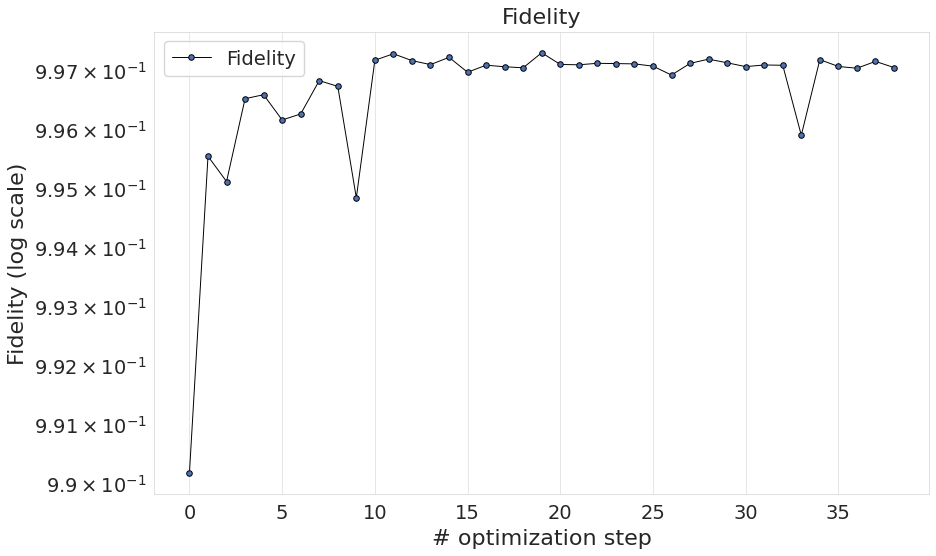
\includegraphics[width=\textwidth]{figures/png/RB_optimization/NM/post_ft_true/NM_fid.png}
        \caption{Plot of the average Clifford gate fidelity as a function of the function evaluations.}
        \label{NM_true_fig:fidelity}
    \end{subfigure}
    \hfill
    \begin{subfigure}[t]{0.495\textwidth}
        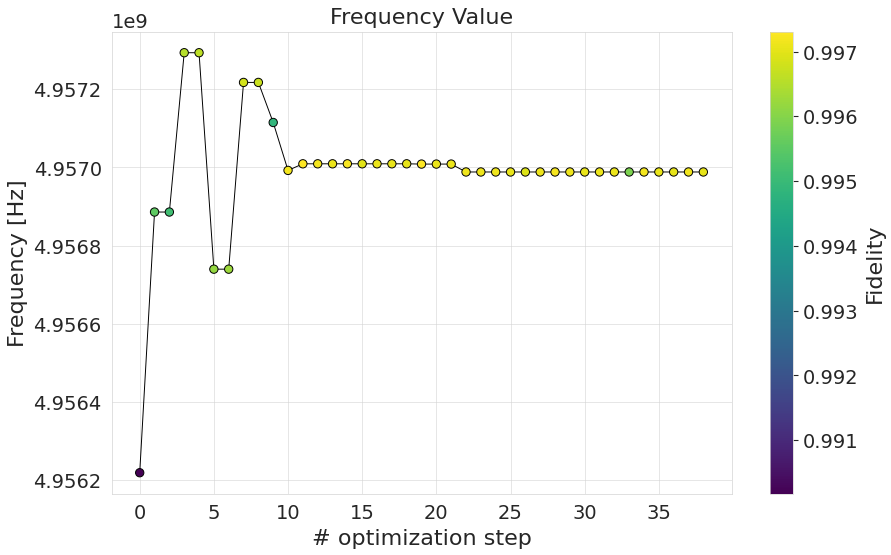
\includegraphics[width=\textwidth]{figures/png/RB_optimization/NM/post_ft_true/frequency.png}
        \caption{Plot of the frequency of the $R_X(\pi)$ gate corresponding to different optimization steps.}
        \label{NM_true_fig:frequency}
    \end{subfigure}

    \vspace{0.5cm}

    \begin{subfigure}[t]{0.495\textwidth}
        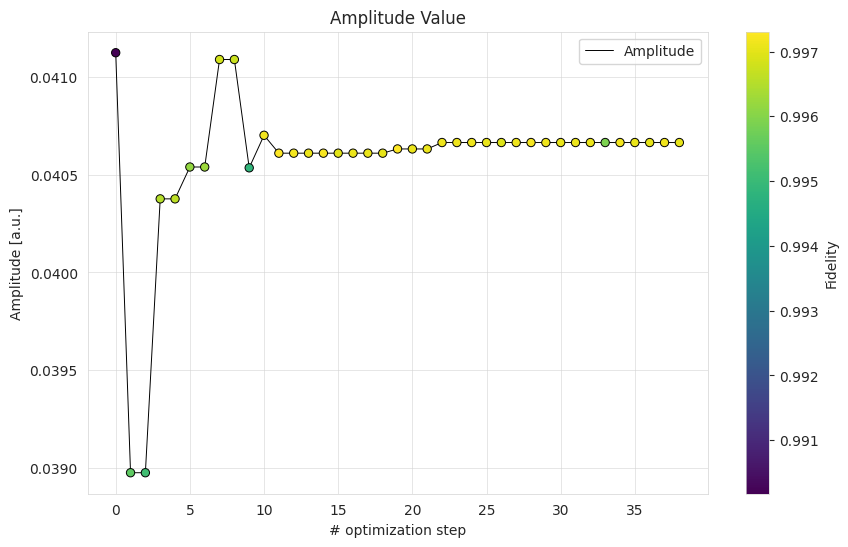
\includegraphics[width=\textwidth]{figures/png/RB_optimization/NM/post_ft_true/amplitude.png}
        \caption{Plot of the amplitude of the $R_X(\pi)$ gate corresponding to different optimization steps.}
        \label{NM_true_fig:amplitude}
    \end{subfigure}
    \hfill
    \begin{subfigure}[t]{0.495\textwidth}
        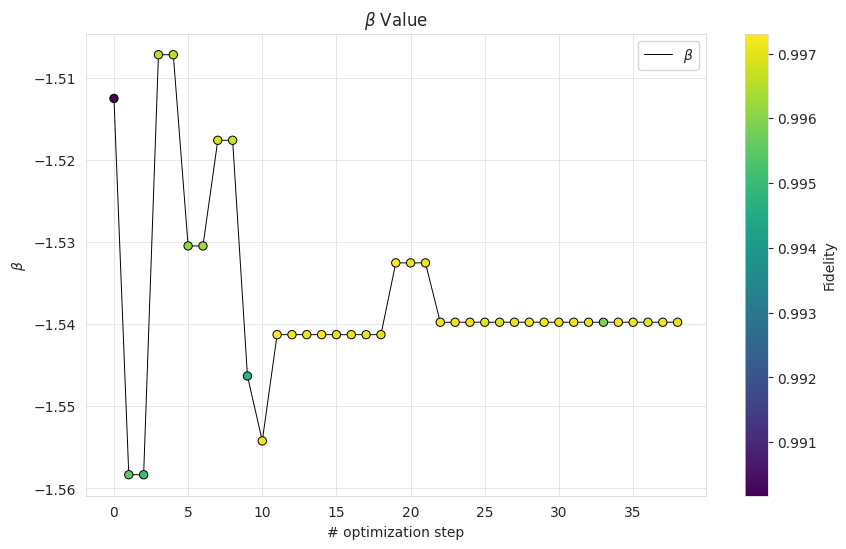
\includegraphics[width=\textwidth]{figures/png/RB_optimization/NM/post_ft_true/beta.png}
        \caption{Plot of the $\beta$ multiplying coefficient for the second quadrature component of the DRAG pulse.}
        \label{NM_true_fig:beta}
    \end{subfigure}

    \caption{Plots of the fidelity and optimization parameters as a function of the number of optimization step.}
    \label{fig:NM_plots}
\end{figure}

The values of the parameters being optimized are reported in Figures \ref{NM_true_fig:frequency}, \ref{NM_true_fig:amplitude}, and \ref{NM_true_fig:beta}. 
From these plots, it is again evident that the optimization is converging as the parameters stabilize around specific values: \texttt{amplitude} $= 0.04$, \texttt{frequency} $= 4.957$ GHz, and \texttt{beta} $= -1.54$.

However, a possible limitation to the performance of this optimization approach may lie in the absence of an explicitly defined initial simplex.
Setting only the initial parameter values, without specifying the full simplex, can lead the algorithm to explore the parameter space inefficiently. 
For this reason, further runs of the same method were carried out, this time also initializing the simplex explicitly.

Furthermore, considering that the allowed variation range for the $\beta$ parameter was restricted to only $\pm0.25$ around the value determined by the \tt{drag\_tuning} routine, quite a small interval, we explored the possibility of improving the efficiency of the optimization by reducing the number of free parameters. 
Specifically, additional optimization runs were performed in which only the amplitude and frequency of the $R_X(\pi)$ pulse were optimized, while $\beta$ was kept fixed at $0$.

This choice was motivated by the working assumption that, at least in this initial phase, leakage errors were not the dominant source of infidelity. 
Since the DRAG correction primarily addresses leakage to higher energy levels, we thought that $\beta$ would have a limited effect on the overall gate fidelity compared to the more significant impact of accurately calibrating the native gate's amplitude and frequency. 
As such, the focus was placed on parameters expected to yield the greatest improvements in fidelity while maintaining a limited run time.

Some optimization runs were performed with this revised configuration, in this case, the initial simplex was constructed based on preliminary fine-tuning routines. 
Specifically, we considered the uncertainties on amplitude and frequency obtained respectively from the flipping and Ramsey procedures.
These values were scaled by a factor of 1.5 to define the characteristic step sizes; using these values, a triangular simplex was generated in the amplitude-frequency parameter space, centered around the initial guess, and offset along each axis to ensure sufficient coverage of the local landscape.

The results of these runs are reported in the following sections and are labeled as \tt{init\_simp\_1}, \tt{init\_simp\_2}, and \tt{init\_simp\_3}.

\begin{figure}[h!]
    \centering
    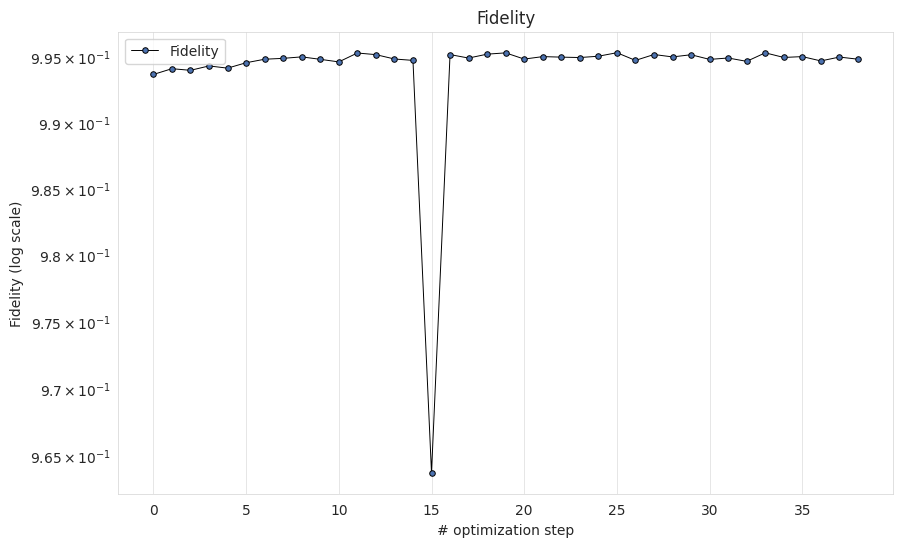
\includegraphics[width=0.495\textwidth]{figures/png/RB_optimization/NM/InitialSymplex/20241110_211211/fidelity.png}
    \caption{Plot of the average Clifford gate fidelity as a function of the optimization steps for the first round optimization - \tt{init\_simp\_1}.}
    \label{fig:20241110_211211:fidelity}
\end{figure}

\begin{figure}[h!]
    \centering
    \begin{subfigure}[t]{0.495\textwidth}
        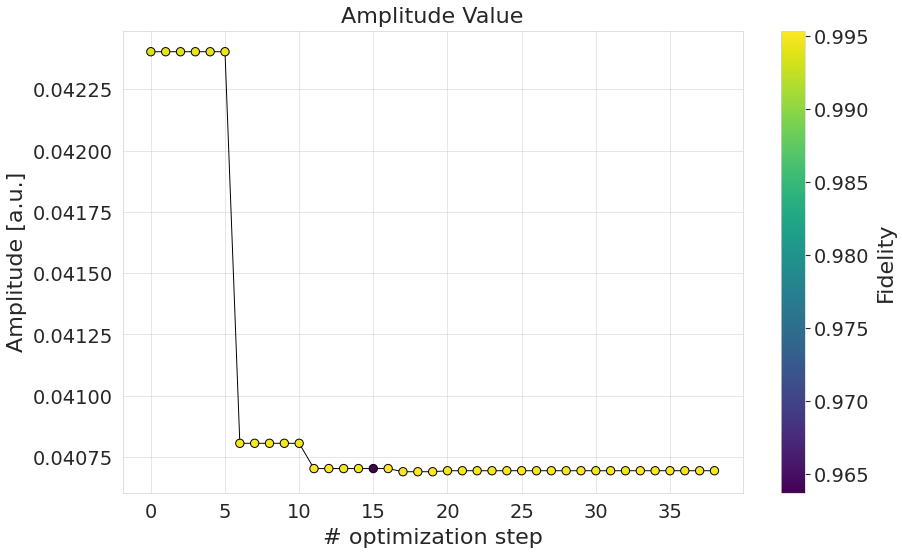
\includegraphics[width=\textwidth]{figures/png/RB_optimization/NM/InitialSymplex/20241110_211211/amplitude.png}
        \caption{Plot of the amplitude of the $R_X(\pi)$ gate corresponding to different optimization steps.}
        \label{fig:20241110_211211:amplitude}
    \end{subfigure}
    \hfill
    \begin{subfigure}[t]{0.495\textwidth}
        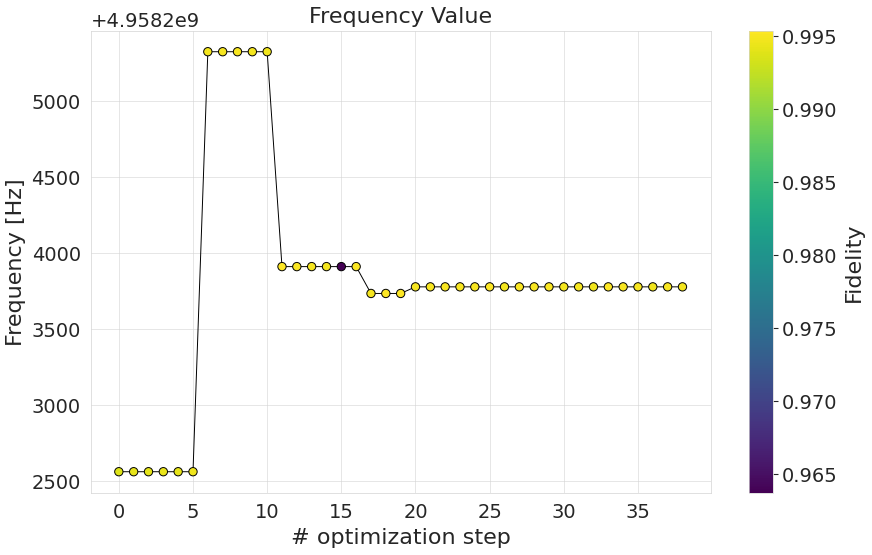
\includegraphics[width=\textwidth]{figures/png/RB_optimization/NM/InitialSymplex/20241110_211211/frequency.png}
        \caption{Plot of the frequency of the $R_X(\pi)$ gate corresponding to different optimization steps.}
        \label{fig:20241110_211211:frequency}
    \end{subfigure}
    \caption{Plots of the optimization parameters as a function of the number of optimization steps for the first round optimization - \tt{init\_simp\_2}.}
    \label{fig:20241110_211211:parameters}
\end{figure}

From the plots showing the outcome of the first optimization run, it can be observed that the fidelity increases over the initial iterations and then stabilizes around a value of approximately 99.45\% after about fifteen steps.
Two aspects are particularly noteworthy. The first concerns the noticeable drop in fidelity observed at the sixteenth iteration, where the fidelity falls below the 97\% threshold (Figure \ref{fig:20241110_211211:fidelity}), despite the amplitude and frequency of the $R_X(\pi)$ pulse showing no significant changes compared to the previous optimization steps (see Figure \ref{fig:20241110_211211:parameters}).
Similar behavior is observed in other plots illustrating the optimization progress for this algorithm (see Figure \ref{fig:20241113_181711:fidelity}), which may point to possible issues in measurement or data acquisition, or to imperfect control over the qubit state.

\begin{figure}[h!]
    \centering
    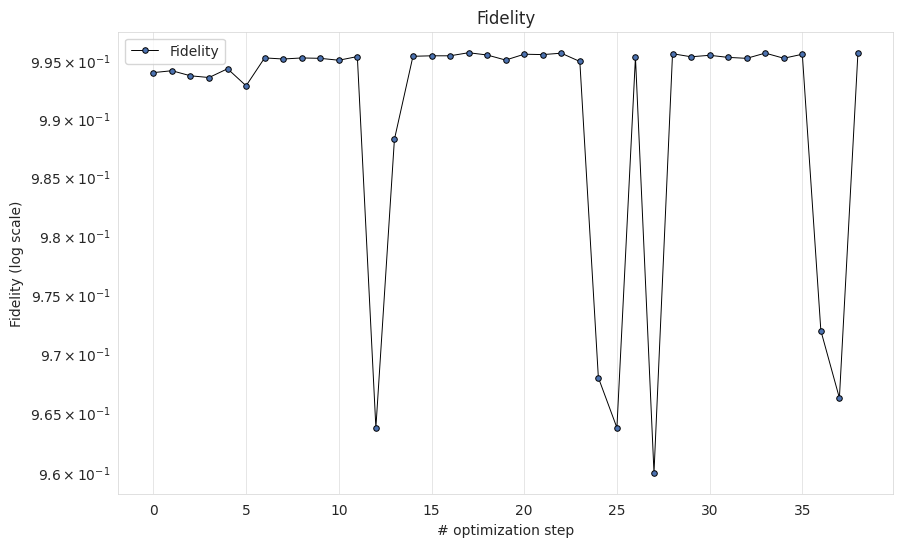
\includegraphics[width=0.495\textwidth]{figures/png/RB_optimization/NM/InitialSymplex/20241113_181711/fidelity.png}
    \caption{Plot of the average Clifford gate fidelity as a function of the optimization steps for the second round optimization - \tt{init\_simp\_2}.}
    \label{fig:20241113_181711:fidelity}
\end{figure}

\begin{figure}[h!]
    \centering
    \begin{subfigure}[t]{0.495\textwidth}
        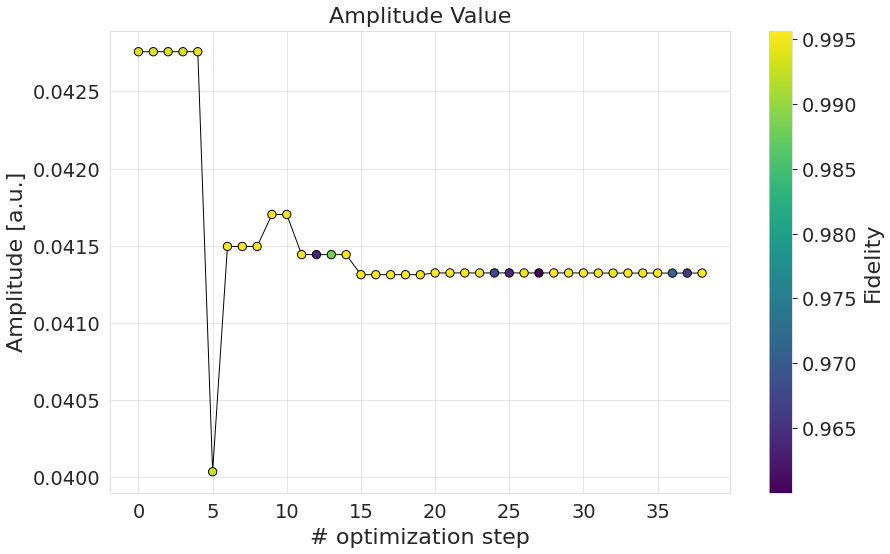
\includegraphics[width=\textwidth]{figures/png/RB_optimization/NM/InitialSymplex/20241113_181711/Amplitude.png}
        \caption{Plot of the amplitude of the $R_X(\pi)$ gate corresponding to different optimization steps.}
        \label{fig:20241113_181711:amplitude}
    \end{subfigure}
    \hfill
    \begin{subfigure}[t]{0.495\textwidth}
        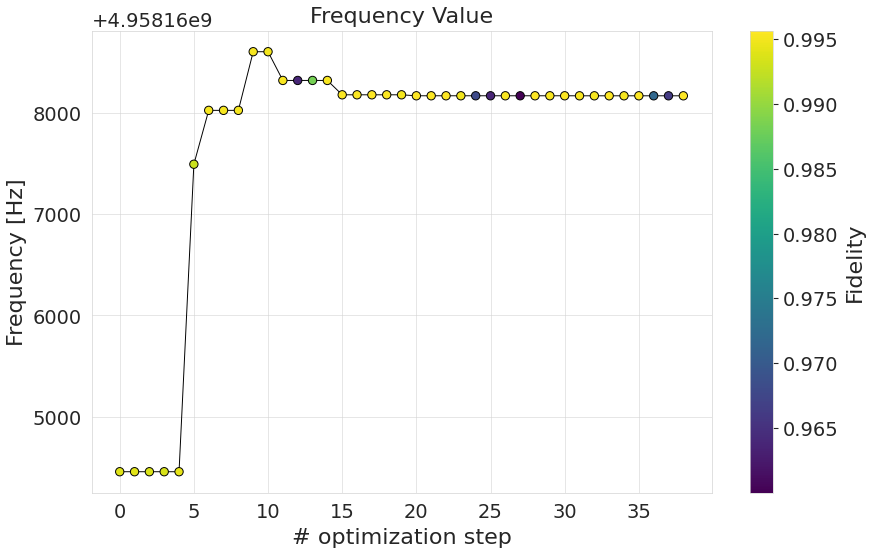
\includegraphics[width=\textwidth]{figures/png/RB_optimization/NM/InitialSymplex/20241113_181711/Frequency.png}
        \caption{Plot of the frequency of the $R_X(\pi)$ gate corresponding to different optimization steps.}
        \label{fig:20241113_181711:frequency}
    \end{subfigure}
    \caption{Plots of the optimization parameters as a function of the number of optimization steps for the first round optimization - \tt{init\_simp\_2}.}
    \label{fig:20241113_181711:parameters}
\end{figure}

In particular, regarding the optimization labeled as \tt{init\_simp\_2}, the most important observation is again the presence of large variations in fidelity despite nearly fixed parameters. 
That is, for comparable values of amplitude and frequency, significantly different fidelity outcomes are observed.
This is especially evident when examining the optimization steps corresponding to the pronounced fidelity dips in Figure \ref{fig:20241113_181711:fidelity}.
By comparing those same steps with the parameter evolution shown in Figure \ref{fig:20241113_181711:parameters}, it becomes evident that neither the amplitude nor the frequency of the $R_X(\pi)$ pulse changes significantly. 
It should be noted, as will be discussed in more detail in the conclusions, that this behavior may ultimately limit the effectiveness of the optimization process in improving the average Clifford gate fidelity. 

\begin{figure}[h!]
    \centering
    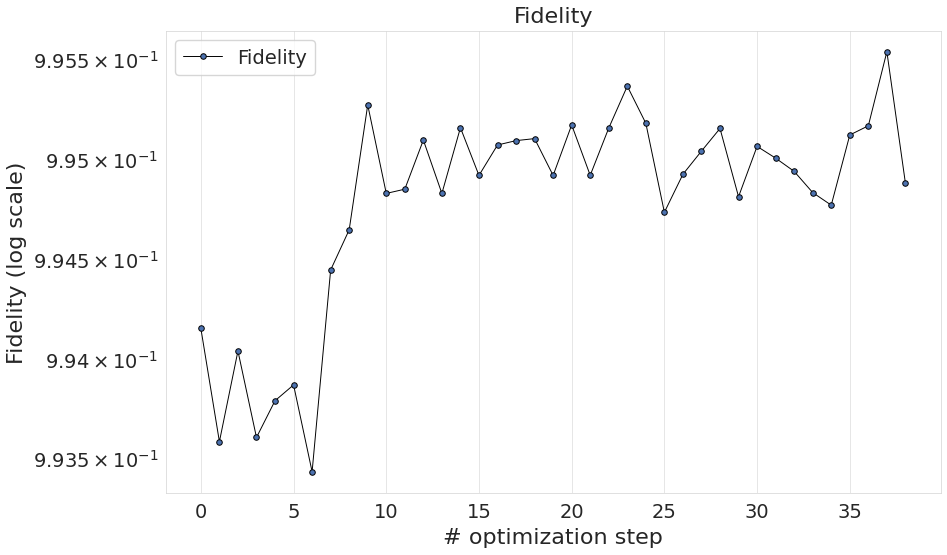
\includegraphics[width=0.495\textwidth]{figures/png/RB_optimization/NM/InitialSymplex/20241113_200745/fidelity.png}
    \caption{Plot of the average Clifford gate fidelity as a function of the optimization steps for the first round optimization - \tt{init\_simp\_3}.}
    \label{fig:20241113_200745:fidelity}
\end{figure}

\begin{figure}[h!]
    \centering
    \begin{subfigure}[t]{0.495\textwidth}
        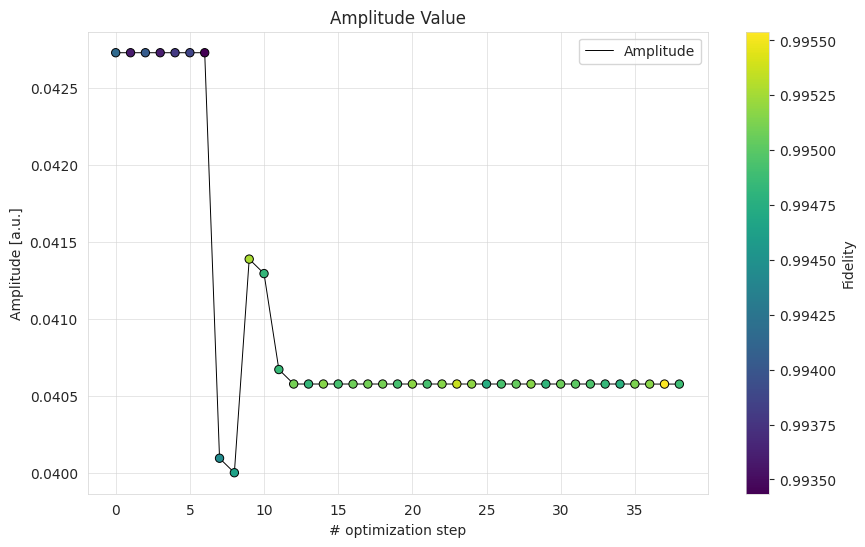
\includegraphics[width=\textwidth]{figures/png/RB_optimization/NM/InitialSymplex/20241113_200745/Amplitude.png}
        \caption{Plot of the amplitude of the $R_X(\pi)$ gate corresponding to different optimization steps.}
        \label{fig:20241113_200745:amplitude}
    \end{subfigure}
    \hfill
    \begin{subfigure}[t]{0.495\textwidth}
        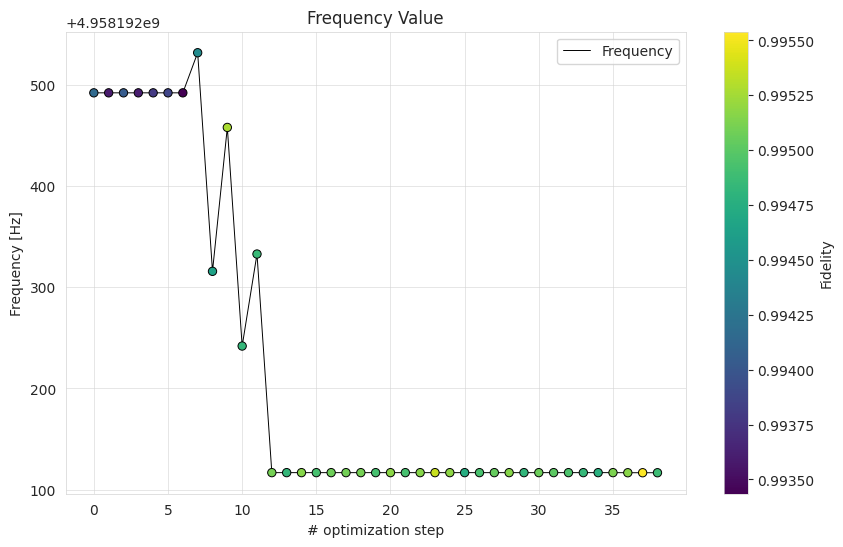
\includegraphics[width=\textwidth]{figures/png/RB_optimization/NM/InitialSymplex/20241113_200745/Frequency.png}
        \caption{Plot of the frequency of the $R_X(\pi)$ gate corresponding to different optimization steps.}
        \label{fig:20241113_200745:frequency}
    \end{subfigure}
    \caption{Plots of the optimization parameters as a function of the number of optimization steps for the first round optimization - \tt{init\_simp\_3}.}
    \label{fig:20241113_200745:parameters}
\end{figure}

In the third and final case, the lack of convergence is apparent directly from the fidelity plot shown in Figure \ref{fig:20241113_200745:fidelity}.
Upon closer inspection, it was observed that the frequency parameter quickly settles at the lower bound of its defined range. 
This initially led to the hypothesis that the preceding Ramsey-based fine-tuning step used to initialize the optimization had failed.
However, this assumption was disproven by the report automatically generated for each operation performed with \Qibocal.
The corresponding Ramsey experiment, which confirms successful execution, is shown in Figure \ref{fig:Ramsey_NM}.
These findings lead us to conclude that in this case, the Nelder Mead algorithm simply failed to converge with the same stability observed in the previous optimization runs.

\begin{figure}[h!]
    \centering
    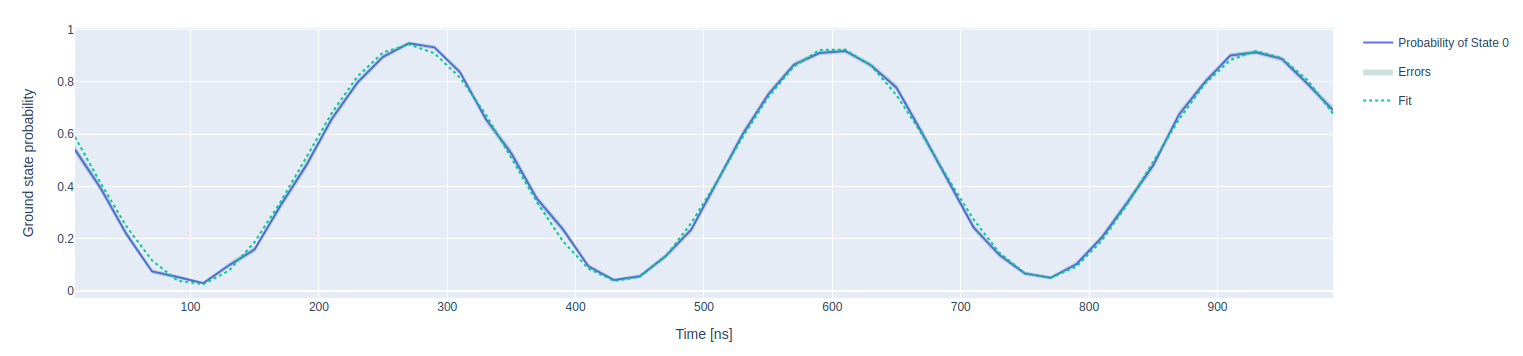
\includegraphics[width=\textwidth]{figures/png/RB_optimization/NM/InitialSymplex/20241113_200745/Ramsey.png}
    \caption{Ramsey experiment performed to fine-tune the $R_X(\pi)$ gate frequency before the optimization process.}
    \label{fig:Ramsey_NM}
\end{figure}

A summary of the results obtained using the Nelder Mead algorithm under different configurations is presented in the top rows of Table \ref{tab:scipy_opt} while a more detailed summary is reported in Table \ref{tab:best_values} and Table \ref{tab:final_values}, at the end of the present chapter.

Overall, it is evident that including the $\beta$ parameter for DRAG correction in the optimization process enabled the achievement of higher average Clifford gate fidelities. 
For this reason, the optimization of $\beta$ was reintroduced in the subsequent optimization attempts.

\subsection{SLSQP}
\subsubsection{Algorithm description}
To explore possible improvements in performance, we tried using a gradient-based algorithm. 
In particular, we used the Sequential Least Squares Programming (SLSQP) method available in the \texttt{SciPy} library.

The Sequential Least Squares Programming (SLSQP) method, originally developed by Dieter Kraft in 1988 \cite{kraft1988slsqp}, is a gradient-based algorithm for solving constrained nonlinear optimization problems.
The algorithm solves a nonlinear constrained problem of the form:
\begin{align*}
& \min_{x \in \mathbb{R}^n} \quad && f(x) \\
& \text{subject to} \quad && c_i(x) = 0, \quad i = 1, \dots, m \\
& && d_j(x) \geq 0, \quad j = 1, \dots, p \\
& && \mathbf{x}^{(L)} \leq \mathbf{x} \leq \mathbf{x}^{(U)}\\
\end{align*}

It belongs to the class of Sequential Quadratic Programming (SQP) methods, which iteratively solve a sequence of quadratic programming subproblems that locally approximate the original nonlinear problem. 
\begin{enumerate}
    \item Linearization: At iteration $k$, the nonlinear constraints are approximated by their first-order Taylor expansion around the current point $\mathbf{x}_k$.
    This transforms the nonlinear constraints into a linear system locally.
    \item Quadratic subproblem construction: The objective is approximated by a quadratic model of the Lagrangian function: \begin{equation}
        \mathcal{L}(\mathbf{x}, \lambda, \mu) = f(\mathbf{x}) - \sum_{i=1}^{m} \lambda_i c_i(\mathbf{x}) - \sum_{j=1}^{p} \mu_j d_j(\mathbf{x}),
    \end{equation}
    where $\lambda_i$ and $\mu_j$ are Lagrange multipliers. 
    The Hessian of the Lagrangian is not computed explicitly but approximated using a BFGS-like quasi-Newton update.
    \item QP Subproblem solution: A quadratic program is solved to determine a search direction $\mathbf{p}_k$, subject to the linearized constraints and bounds. 
    The subproblem minimizes the quadratic model subject to these constraints.
    \item Constrained line search: A line search is performed along $\mathbf{p}_k$ using a merit function that balances reduction in the objective with the feasibility of constraints. 
    This helps ensure global convergence.
    \item Update: The iterate is updated via $\mathbf{x}_{k+1} = \mathbf{x}_k + \alpha_k \mathbf{p}_k$, where $\alpha_k$ is the step size determined by the line search. 
    The quasi-Newton approximation of the Hessian is also updated.
    \item Termination: The algorithm terminates when the norm of the projected gradient and constraint violations fall below a specified tolerance.
\end{enumerate}

If analytic derivatives for the objective or constraints are not provided, they are approximated using forward finite differences. 
In such cases, each gradient estimation requires $n+1$ function evaluations per iteration, where $n$ is the number of variables.
The values of internal parameters, such as merit function balancing terms and quasi-Newton updates, are managed internally and are not user-configurable through \tt{SciPy}.

\subsubsection{Results}
As shown in Figure \ref{fig:SLSQP:fidelity}, the optimization procedure appears to converge, a result that is also confirmed by the object returned by the \texttt{SciPy} optimizer.
This indicates that the algorithm successfully reached a local minimum within the specified tolerance of $1\cdot10^{-4}$ in less the 15 optimization steps. On the other hand, it is important to consider that SLSQP is a gradient-based method and, as such, may lack robustness in the presence of a noisy or irregular cost landscape.
This makes it susceptible to becoming trapped in local minima, especially if the optimization is not ideal.

For this run, the same constraints and parameter bounds used in the Nelder-Mead optimization were applied: a maximum of 40 optimization steps and parameter ranges set by the initial fine-tuning routine carried out before the fidelity optimization.

\begin{figure}[h]
    \centering
    \begin{subfigure}[t]{0.495\textwidth}
        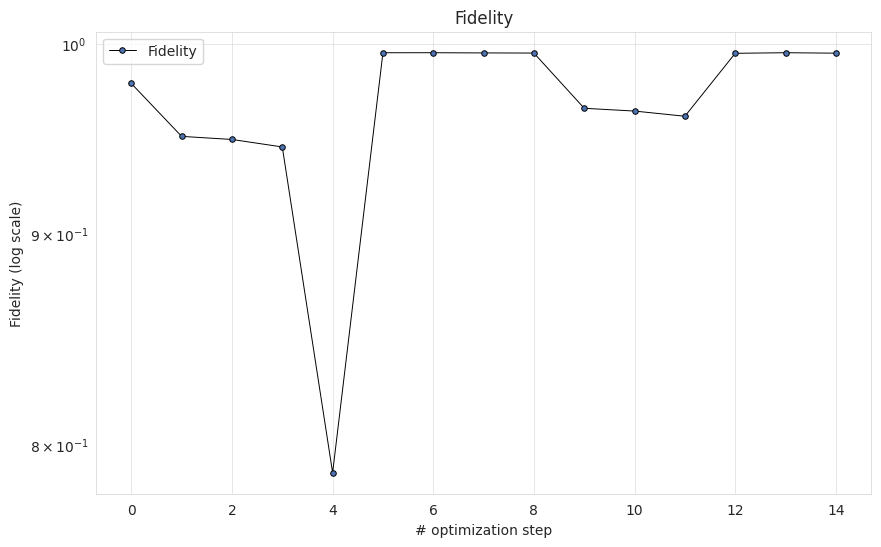
\includegraphics[width=\textwidth]{figures/png/RB_optimization/SLSQP/fidelity.png}
        \caption{Plot of the average Clifford gate fidelity as a function of the optimization steps.}
        \label{fig:SLSQP:fidelity}
    \end{subfigure}
    \hfill
    \begin{subfigure}[t]{0.495\textwidth}
        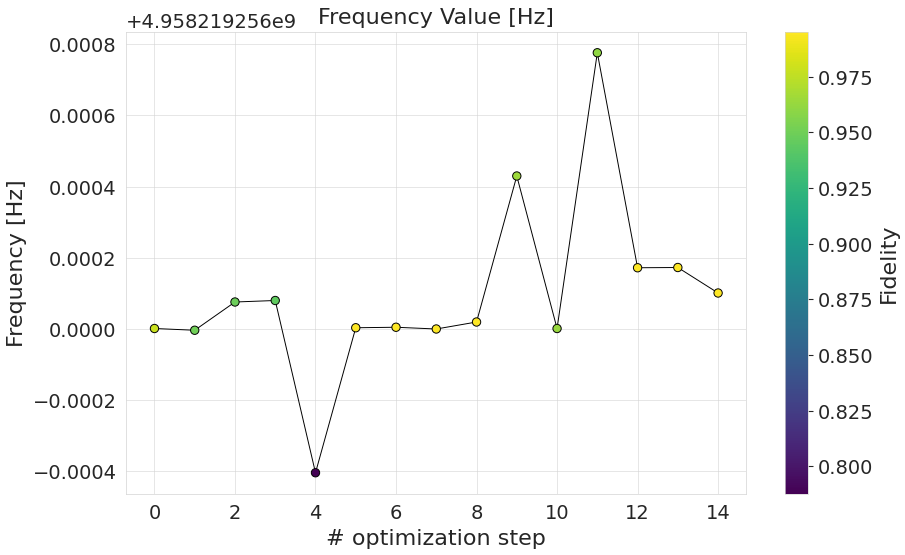
\includegraphics[width=\textwidth]{figures/png/RB_optimization/SLSQP/frequency.png}
        \caption{Plot of the frequency of the $R_X(\pi)$ gate corresponding to different optimization steps.}
        \label{fig:SLSQP:frequency}
    \end{subfigure}

    \vspace{0.5cm}

    \begin{subfigure}[t]{0.495\textwidth}
        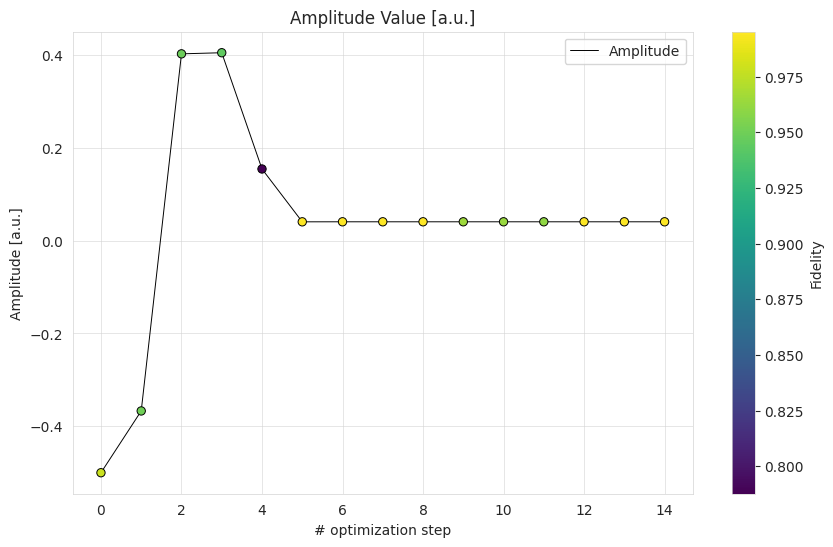
\includegraphics[width=\textwidth]{figures/png/RB_optimization/SLSQP/amplitude.png}
        \caption{Plot of the amplitude of the $R_X(\pi)$ gate corresponding to different optimization steps.}
        \label{fig:SLSQP:amplitude}
    \end{subfigure}
    \hfill
    \begin{subfigure}[t]{0.495\textwidth}
        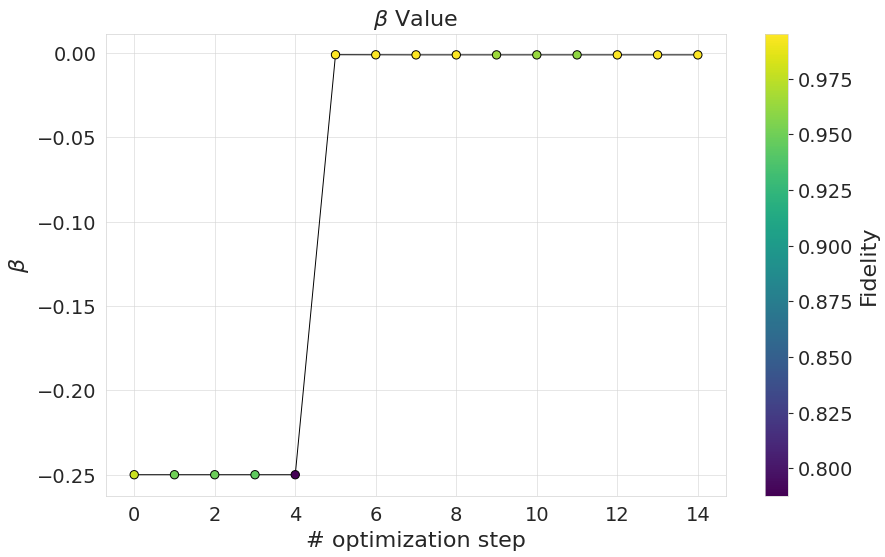
\includegraphics[width=\textwidth]{figures/png/RB_optimization/SLSQP/beta.png}
        \caption{Plot of the $\beta$ multiplying coefficient for the second quadrature component of the DRAG pulse.}
        \label{fig:SLSQP:beta}
    \end{subfigure}

    \caption{Plots of the fidelity and optimization parameters as a function of the number of optimization steps for the SLSQP optimization method.}
    \label{fig:SLSQP_plots}
\end{figure}

In this case, an interesting observation is that, as expected, a sharp drop in fidelity corresponds to a frequency value that deviates significantly from the optimal one for the $R_X(\pi)$ gate.
This behavior is consistent with the assumption that frequency and amplitude are the two dominant parameters in determining the quality of the $R_X(\pi)$ gate and as a consequence the average fidelity of Clifford gates.

However, as can be seen in Figure \ref{fig:SLSQP:fidelity}, the convergence behavior is not particularly stable: the fidelity exhibits large step-to-step fluctuations. 
As mentioned previously, this indicates that the SLSQP method is not robust enough to be reliably used as a systematic approach for optimizing average Clifford gate fidelity.
In particular, it becomes difficult to define a minimum number of steps beyond which a certain fidelity level can be guaranteed.

Furthermore, from a computational standpoint, this method is relatively inefficient. 
Since the gradient must be estimated numerically, each step involves multiple evaluations of the cost function, significantly increasing the total number of function calls required (see Table \ref{tab:scipy_opt}).

\begin{table}[h]
    \centering
    \begin{tabular}{lcccccc}
        \toprule
        \textbf{Method} & \textbf{Success} & \textbf{Infidelity} & \textbf{Iterations} & \textbf{RB Evaluations} & \textbf{Duration [s]}\\
        \midrule
        \textbf{Nelder-Mead} & False & 0.002732 & 40 & 93 & 2892 \\
        \textbf{init\_simplex\_1} & False &  0.004593 & 40 & 99 & 3096\\
        \textbf{init\_simplex\_2} & False & 0.004297 & 40 & 100 & 3128\\
        \textbf{init\_simplex\_3} & False & 0.004507 & 40 & 106 & 3190\\
        \textbf{SLSQP} & True & 0.004861 & 15 & 180 & 3873\\
        \bottomrule
    \end{tabular}
    \caption{This table provides a short summary of the results obtained using different optimization methods available in \texttt{SciPy}.\\ 
    The \textit{Success} column indicates whether the algorithm converged successfully. 
    A value of True denotes that convergence was achieved within the specified tolerance of $1\cdot10^{-4}$ and before reaching the maximum number of iterations; otherwise, the value is False.\\
    The reported value of the objective function corresponds to the average Clifford gate infidelity obtained at the end of optimization via Randomized Benchmarking (1-fidelity), which serves as the cost function minimized by the algorithm.
    The \textit{Duration} column refers to the total runtime of the script, including the initial fine-tuning stage preceding the optimization.\\}
    \label{tab:scipy_opt}
\end{table}


\section{CMA-ES}

\subsection{Algorithm description}\label{sec:CMA}
Covariance Matrix Adaptation Evolution Strategy (\tt{CMA-ES} \cite{cmaessimplepractical}), is a population-based evolutionary algorithm designed for optimizing complex, non-convex, and high-dimensional functions.\\
It belongs to the broader class of Evolution Strategies (ES), a subset of Evolutionary Algorithms (EAs)(see \cite{sloss20192019evolutionaryalgorithmsreview}), and is particularly effective for black-box optimization where gradient information is unavailable.

Evolution Strategies (ES) are a class of optimization methods that employ self-adaptive mechanisms to explore the search space efficiently. 
Unlike classical optimization techniques that rely on gradient descent, ES leverages stochastic sampling to navigate rugged and multimodal landscapes.
In this context, \tt{CMA-ES} is an adaptive stochastic search method that iteratively refines a probability distribution over the search space. 
Unlike traditional Genetic Algorithms (GAs), which rely on crossover and mutation operators, \tt{CMA-ES} employs a multivariate normal distribution to generate candidate solutions. 
The method adaptively updates the distribution's mean and covariance matrix based on the fitness of sampled points.

The fundamental idea behind \tt{CMA-ES} is the use of a multivariate Gaussian distribution to model promising search directions. 
Let $\mathbf{\mu}_t$ denote the mean of the distribution at iteration $t$, and $\Sigma_t$ the covariance matrix. 
Then, a new population of $\lambda$ candidate solutions $\mathbf{x}_i^{(t+1)} \sim \mathbf{\mu}_t + \sigma_t\mathcal{N}(\mathbf{\mu}_t,\mathbf{\sigma}_t^2, \Sigma_t)$, where $\sigma_t$ is a step size controlling the exploration.  

The \tt{CMA-ES} algorithm follows the following steps:\begin{enumerate}
    \item If not otherwise specified, the initial parameters are set: mean vector $\mathbf{\mu_0}$, covariance matrix $\Sigma_0$\footnote{$\Sigma_0=\mathbb{I}$ for isotropic search}, step size $\sigma_0$, population size $\lambda$
    \item Generate $\lambda$ new candidate solutions $\mathbf{x}_i$ according to a multivariate normal distribution.
    \item Evaluate the objective function $f(\mathbf{x}_i)$ for each candidate solution.
    \item Sort the new candidate solutions based on fitness: $f(\mathbf{x}_0) \leq ... \leq f(\mathbf{x}_{\lambda})$.
    \item Update the mean vector $\mathbf{\mu}$ with the $m=\lfloor \lambda / 2 \rfloor$ top performing solutions:\begin{equation}
        \mathbf{\mu} \leftarrow \sum_{i=0}^m \mathbf{w}_i\mathbf{x}_i,
    \end{equation} where $\mathbf{w}_i$ are internally defined weights.
    \item Update the isotropic and anisotropic evolution path $\mathbf{p}_{\sigma}$, $\mathbf{p}_c$ \footnote{For details on the update process of the evolution paths see \cite{cmaessimplepractical}.}.
    \item Update the covariance matrix: \begin{equation}
        C \leftarrow (1 - c_1 - c_{\mu}) C + c_1 \mathbf{p}_c \mathbf{p}_c^T + c_{\mu} \sum_{i=1}^{\mu} w_i \mathbf{y}_i \mathbf{y}_i^T,
    \end{equation} where $c_1$ and $c_\mu$ are learning rates and $\mathbf{y}_i$ represents the deviation of the $i$-th candidate solution from the mean $\mathbf{mu}$.
    \item Update the step size using a cumulative path evolution mechanism \begin{equation}
        \sigma \leftarrow \sigma \cdot \exp \left( \frac{c_{\sigma}}{d_{\sigma}} \left( \| \mathbf{p}_{\sigma} \| - E \| \mathcal{N}(0, I) \| \right) \right),
    \end{equation} where $c_\sigma$ is the learning rate for step-size adaptation, $d_\sigma$ is a damping factor $\| \mathbf{p}_{\sigma} \|$ is the length of the evolution path and $E \| \mathcal{N}(0, I) \|$ is the expected length of a standard normally distributed random vector.
\end{enumerate}

We decided to test \tt{CMA-ES} for the RB optimization as it is particularly well-suited for noisy or non-smooth objective functions. 
The stochastic nature of \tt{CMA-ES} allows it to remain robust against such perturbations, as it does not rely on local gradient information and instead, samples across a distribution to infer promising search directions.

Unless manually specified, \tt{CMA-ES} employs internal heuristics to determine several of its hyperparameters. 
For instance, the population size $\lambda$ is typically set according to the dimensionality of the problem:
\begin{equation}\label{eq:pop_size}
    \lambda = 4+3\lfloor \log{n}\rfloor
\end{equation}
where $n$ is the problem dimension \cite{hansen_pycma_2024}.
For full details on default parameter settings and adaptation rules, see \cite{cmaessimplepractical}.

\subsection{Results}

In the \tt{CMA-ES} optimization run, parameter settings were chosen to be as consistent as possible with those used in previous optimization algorithms.
Specifically, the initial values and the parameter bounds were defined as shown in Listing \ref{snippet:params_init}, based on the results of the preliminary fine-tuning procedure. 
The maximum number of generations was set to 30, slightly lower than the iteration limits used in the \texttt{SciPy}-based methods.
This choice was motivated by two main considerations. First, we expected a performance comparable to that of the previously tested algorithms, and that consequently, 30 optimization steps (or generations) would be enough to reach an improved fidelity value.
Second, we expected the algorithm to require longer execution times due to the larger number of cost functions evaluation: the population size was not manually set but allowed to default to the internal rule of the \tt{CMA-ES} implementation, as in Equation \ref{eq:pop_size}.
In this case, with three parameters, pulse amplitude, frequency, and DRAG correction parameter $\beta$, the population consisted of 7 candidate solutions per generation.
Given a population of 7 individuals and a total of 30 generations, the optimization required 210 evaluations of the objective function to complete. 

\begin{figure}[h]
    \centering
    \begin{subfigure}[t]{0.495\textwidth}
        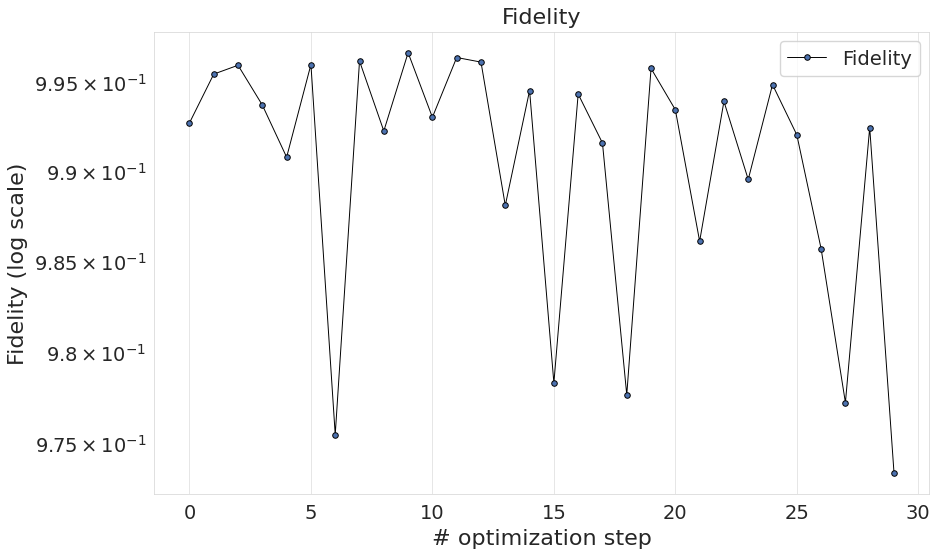
\includegraphics[width=\textwidth]{figures/png/RB_optimization/CMA/fidelity.png}
        \caption{Plot of the average Clifford gate fidelity as a function of the optimization steps.}
        \label{fig:CMA:fidelity}
    \end{subfigure}
    \hfill
    \begin{subfigure}[t]{0.495\textwidth}
        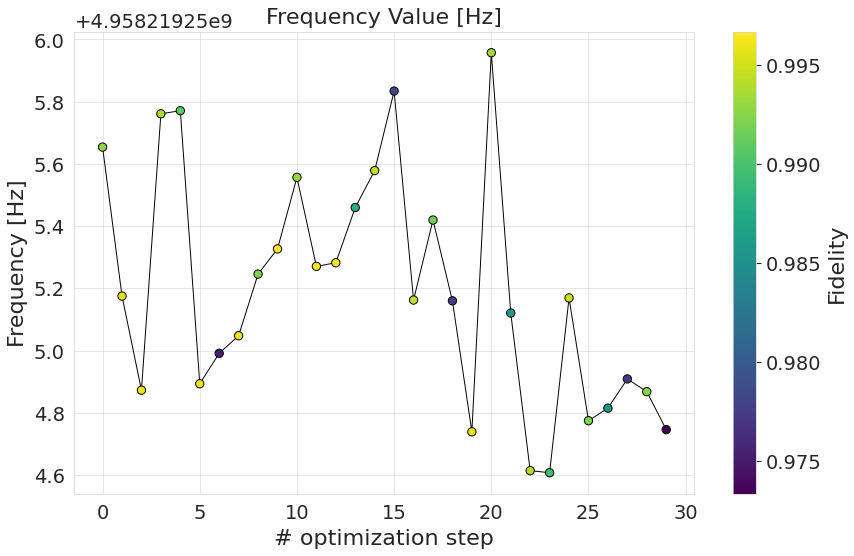
\includegraphics[width=\textwidth]{figures/png/RB_optimization/CMA/CMA_frequency.png}
        \caption{Plot of the frequency of the $R_X(\pi)$ gate corresponding to different optimization steps.}
        \label{fig:CMA:frequency}
    \end{subfigure}

    \vspace{0.5cm}

    \begin{subfigure}[t]{0.495\textwidth}
        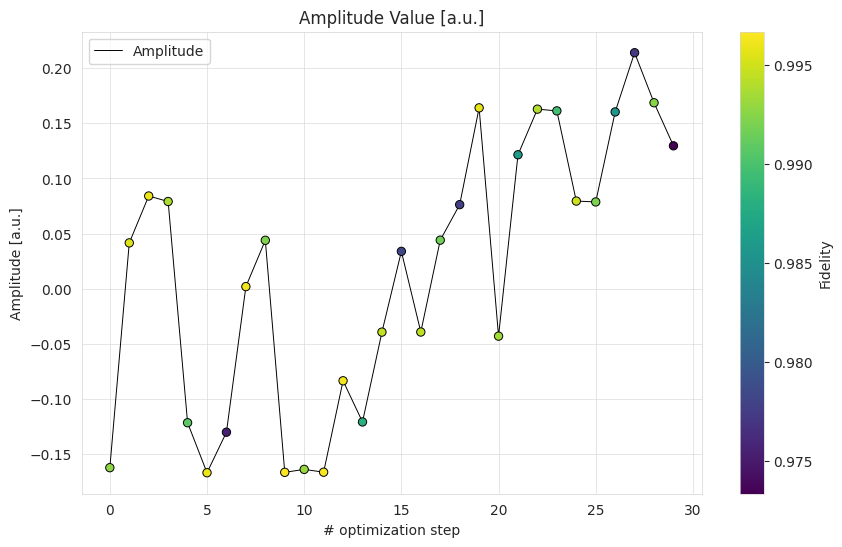
\includegraphics[width=\textwidth]{figures/png/RB_optimization/CMA/CMA_amplitude.png}
        \caption{Plot of the amplitude of the $R_X(\pi)$ gate corresponding to different optimization steps.}
        \label{fig:CMA:amplitude}
    \end{subfigure}
    \hfill
    \begin{subfigure}[t]{0.495\textwidth}
        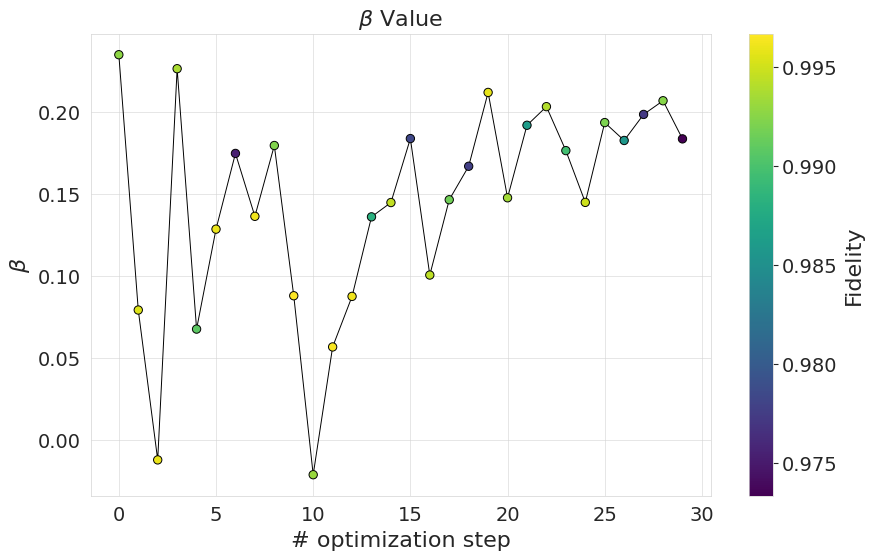
\includegraphics[width=\textwidth]{figures/png/RB_optimization/CMA/beta_CMA.png}
        \caption{Plot of the $\beta$ multiplying coefficient for the second quadrature component of the DRAG pulse.}
        \label{fig:CMA:beta}
    \end{subfigure}

    \caption{Plots of the fidelity and optimization parameters as a function of the number of optimization steps for the CMA optimization method.}
    \label{fig:CMA_plots}
\end{figure}

The results of the fidelity optimization using the \tt{CMA-ES} algorithm are presented in Figure \ref{fig:CMA_plots}. 
Each point in the plots corresponds to the best-performing individual within the population at each of the 30 optimization steps (generations). 
As shown, the algorithm does not achieve full convergence within the allowed number of generations. 
This outcome is likely influenced by the relatively small population size used. 
Indeed, previous studies in the literature have demonstrated that larger populations can significantly improve the performance per function evaluation \cite{hansen2004evaluating}, obviously at the cost of increased computational time.

The choice to limit both the number of generations and the population size was made deliberately to maintain a manageable total runtime. 
Increasing either of these parameters would have led to a substantial rise in computational cost, as \tt{CMA-ES} evaluates the objective function $\lambda$ times per generation where $\lambda$ is the population size.

Another factor that negatively influenced the algorithm convergence is the choice of the initial step size parameter, $\sigma = 0.25$. 
In \tt{CMA-ES} $\sigma$ controls the standard deviation of the multivariate normal distribution used to generate the first population, thereby determining how broadly the algorithm explores the parameter space around the initial guess. 
A smaller $\sigma$ would have concentrated the search in a narrower region, possibly leading to faster convergence to a local optimum. 
However, this value of $\sigma = 0.25$ was chosen with the goal of exploring a wider portion of the parameter space than in previous \texttt{SciPy}-based optimizations, in order to investigate the possible presence of higher-fidelity regions that had not yet been sampled.
An evaluation of the computational cost of running the \tt{CMA-ES} algorithm is reported in Table \ref{tab:optuna_opt}.

\section{Optuna}

\subsection{Algorithm description}

The Tree-Structured Parzen Estimator (TPE) algorithm, as implemented in the \tt{Optuna} optimization framework \cite{optuna_2019}, is a model-based, derivative-free optimization method. 
\tt{Optuna} belongs to the class of Sequential Model-Based Optimization (SMBO) strategies \cite{SMBO_proceedings}, which iteratively refine a surrogate model of the objective function based on past evaluations and select new points in parameter space by balancing exploration and exploitation \cite{BayesianOptimizationReview}.

The TPE method differs from classical Gaussian Process-based Bayesian optimization by using non-parametric density estimation to guide the search through parameter space. 
Instead of directly modeling the objective function $f(\mathbf{x})$, TPE models the conditional probability distribution of the parameters $\mathbf{x}$ given the value of the objective function.

Given a set of past observations $\{ (\mathbf{x}_i, y_i) \}_{i=1}^N$, where $ y_i = f(\mathbf{x}_i) $, the algorithm proceeds as follows:

\begin{enumerate}
    \item Split the observations: Define a threshold value $ y^* $, typically chosen as a quantile of the observed objective values. 
        The dataset is then split into two subsets:
        \begin{itemize}
            \item $\mathcal{L} = \{ \mathbf{x}_i : y_i < y^* \}$, the set of promising configurations
            \item $\mathcal{G} = \{ \mathbf{x}_i : y_i \geq y^* \}$, the set of less promising configurations
        \end{itemize}
    \item Estimate densities: Construct two kernel density estimators (KDEs) to approximate the conditional densities:
    \[
    l(\mathbf{x}) \approx p(\mathbf{x} \mid y < y^*) \quad \text{and} \quad g(\mathbf{x}) \approx p(\mathbf{x} \mid y \geq y^*).
    \]
    \item Candidate sampling: Draw a number of candidate parameter configurations $\mathbf{x}$ from the distribution $l(\mathbf{x})$, which is biased toward more promising regions of the search space.
    \item Acquisition function: For each sampled candidate $\mathbf{x}$, compute the ratio
    \[
    \text{EI}(\mathbf{x}) = \frac{l(\mathbf{x})}{g(\mathbf{x})},
    \]
    which serves as an acquisition function analogous to expected improvement. The candidate with the highest ratio is selected for evaluation.
    \item Evaluate and update: Evaluate the objective function $ y = f(\mathbf{x}) $ at the selected configuration and append the result to the history. Return to step 1.
\end{enumerate}
This process continues until a stopping criterion is met, such as a maximum number of trials or convergence of the best-observed value.

Differently from other TPE implementations, \tt{Optuna} supports automatic pruning designed to terminate unpromising trials early, thus reducing the computational cost. 
In common applications such as neural network training, pruning is enabled by reporting intermediate objective values via \texttt{trial.report(...)} and comparing them to statistics of previously completed trials. 
By default, \texttt{Optuna} employs the \texttt{MedianPruner}, which terminates a trial if its intermediate value is worse than the median of completed trials at the same step.

In the present work, the cost function is defined as the infidelity extracted from a complete RB routine and the optimization problem involves a low-dimensional parameter space, comprising only three continuous parameters; given these characteristics, pruning was not applied.

\subsection{Results}

As a first attempt at applying the optimization algorithm implemented in the \texttt{Optuna} library, a total of 30 optimization steps, or trials as referred to in the library itself, were performed. 
This choice was made to maintain consistency with the number of steps used in previous optimization methods. 
As in the earlier cases, initial parameter values and search boundaries were provided to the algorithm and derived from the fine-tuning routines executed prior to the optimization.

The results obtained with this first optimization attempt are reported in Figure \ref{fig:optuna30:optimization} - \ref{fig:optuna30:beta}.

%30 steps
\begin{figure}[h!]
    \centering
    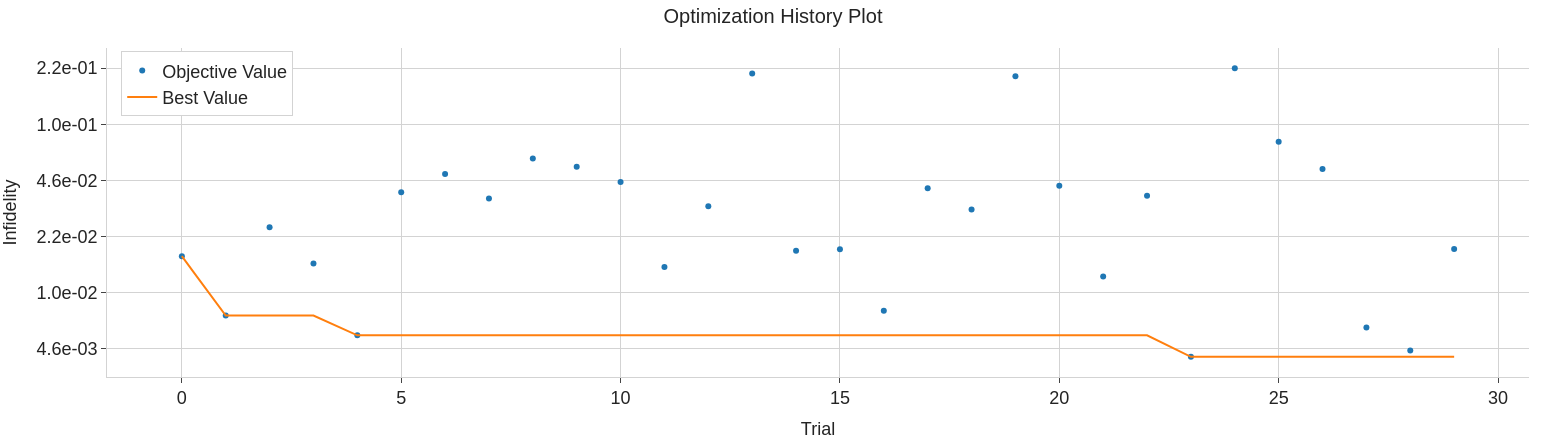
\includegraphics[width=\textwidth]{figures/png/RB_optimization/Optuna/30/optimization.png}
    \caption{Plot of the optimization history using \tt{Optuna} for 30 trials. Infidelity as a function of trials.}
    \label{fig:optuna30:optimization}
\end{figure}

\begin{figure}[h!]
    \centering
    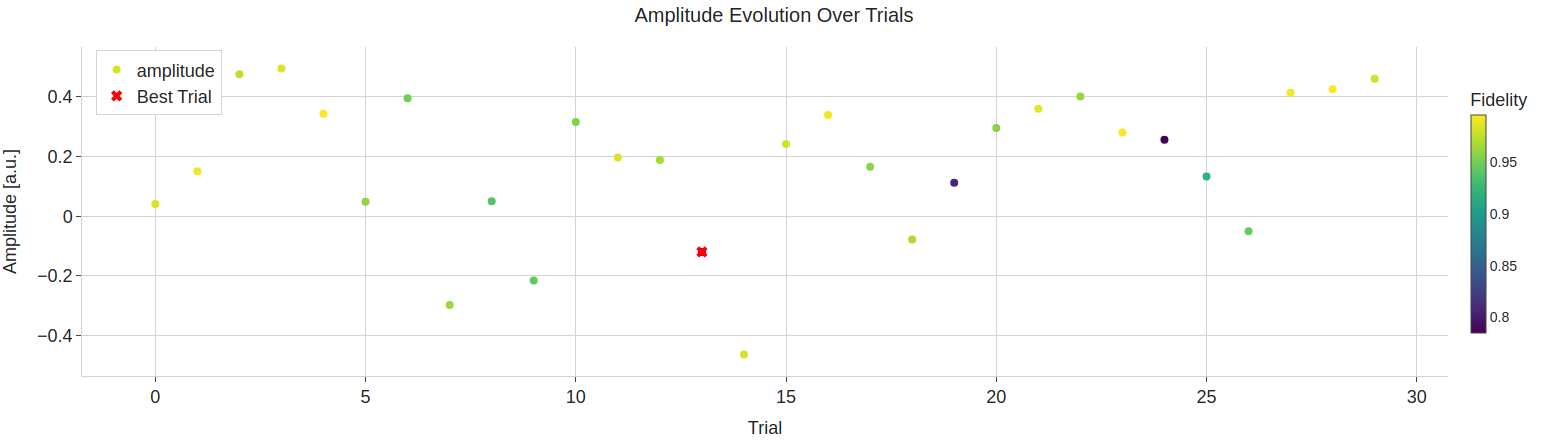
\includegraphics[width=\textwidth]{figures/png/RB_optimization/Optuna/30/amplitude.png}
    \caption{Plot of the $R_X(\pi)$ amplitude as a function of the number of trials.
    The color map indicates the Clifford gate average fidelity.
    The red cross denotes the $R_X(\pi)$ amplitude corresponding to the highest observed fidelity.}
    \label{fig:optuna30:amplitude}
\end{figure}

\begin{figure}[h!]
    \centering
    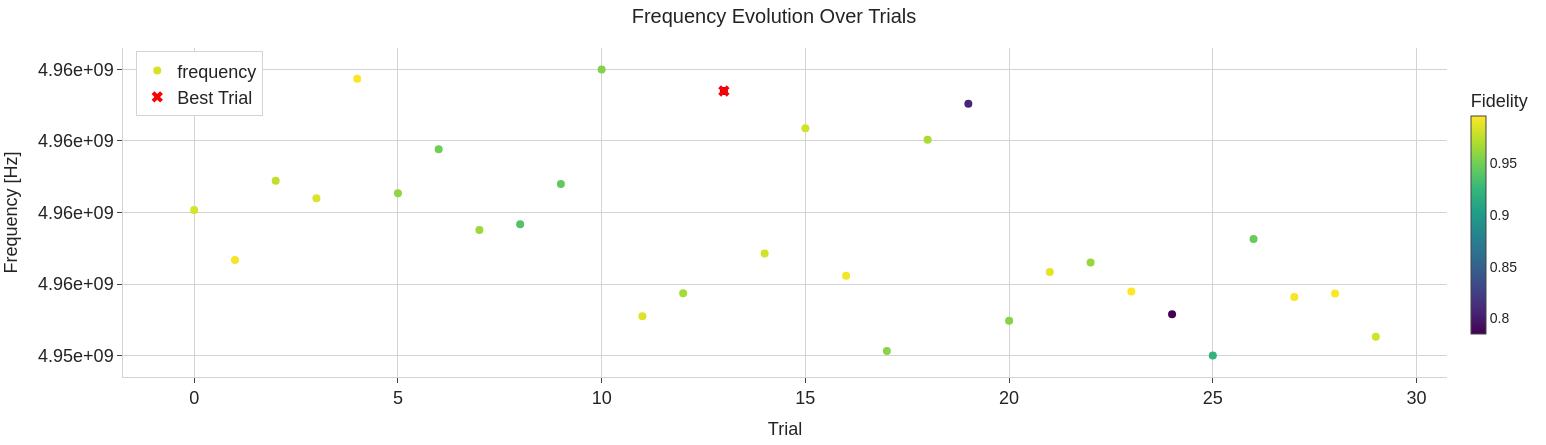
\includegraphics[width=\textwidth]{figures/png/RB_optimization/Optuna/30/frequency.png}
    \caption{Plot of the $R_X(\pi)$ frequency as a function of the number of trials. 
    The color map indicates the Clifford gate average fidelity.  
    The red cross denotes the $R_X(\pi)$ frequency corresponding to the highest observed fidelity}
    \label{fig:optuna30:frequency}
\end{figure}

\begin{figure}[h!]
    \centering
    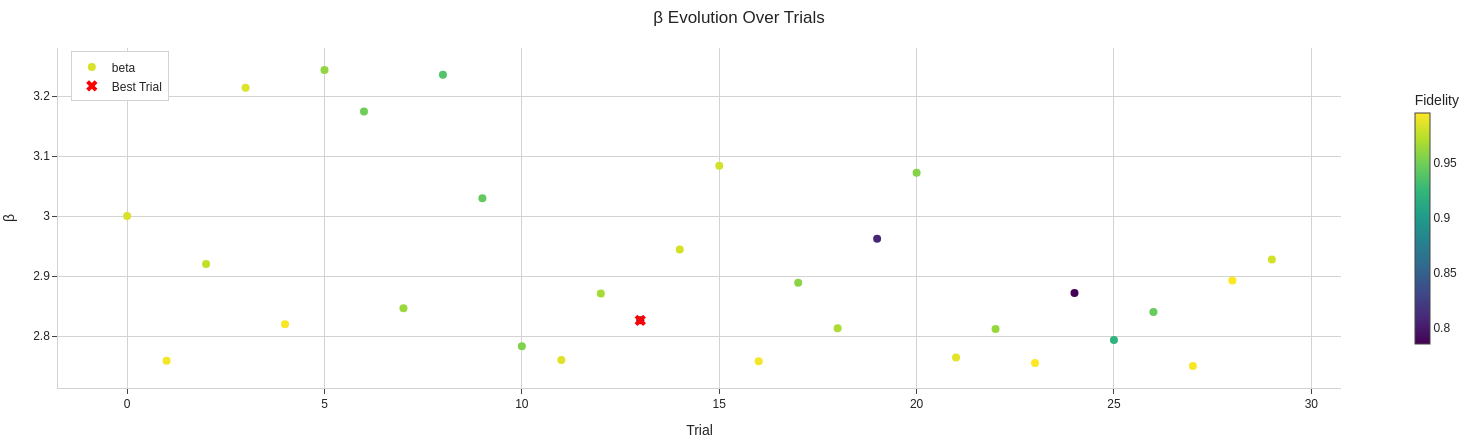
\includegraphics[width=\textwidth]{figures/png/RB_optimization/Optuna/30/beta.png}
    \caption{Plot of the value of the $\beta$ coefficient for the second quadrature of the $R_X(\pi)$ pulse as a function of the number of trials. 
    The color map indicates the Clifford gate average fidelity.  
    The red cross denotes the $\beta$ value corresponding to the highest observed fidelity}
    \label{fig:optuna30:beta}
\end{figure}

The first observation from the optimization plots is that no clear convergence is achieved. 
This behavior is not unexpected and can be attributed to the nature of the \tt{Optuna} optimization framework, which is not designed to guarantee convergence in the traditional sense. 
Unlike gradient-based methods or some evolutionary strategies, \tt{Optuna} is more exploratory by design and may not settle into a stable optimum within a fixed number of trials.

Instead, \tt{Optuna} proves valuable as a tool for systematically exploring the parameter space. 
In doing so, it may identify previously unvisited regions that yield better performance. 
In this specific run, the highest fidelity was achieved at the 23rd trial, reaching an average Clifford gate fidelity of 99.58\%. 
A result that is comparable to the best fidelities obtained using the other optimization strategies tested.

However, a clear advantage of using \tt{Optuna} is its efficiency. 
The entire optimization process, comprising only 30 function evaluations, was completed in approximately 12 minutes; see Table \ref{tab:optuna_opt} for the exact runtime in seconds. 
Due to this relatively low computational cost, it becomes feasible to explore a larger number of trials to assess whether higher fidelities can be achieved or whether the algorithm can exhibit more stable convergence patterns.

Based on this reasoning, a second optimization run was performed using 100 trials. 
The evolution of the fidelity during this extended optimization is shown in Figure \ref{fig:optuna100:optimization}. 
Contrary to initial expectations that a longer optimization would yield better results, it was observed that the lowest cost function value (i.e., highest fidelity) was reached within the first 20 steps. 
In particular, the best average Clifford gate fidelity of 99.64\% was obtained at the 13\textsuperscript{th} trial.

%100 steps
\begin{figure}[h!]
    \centering
    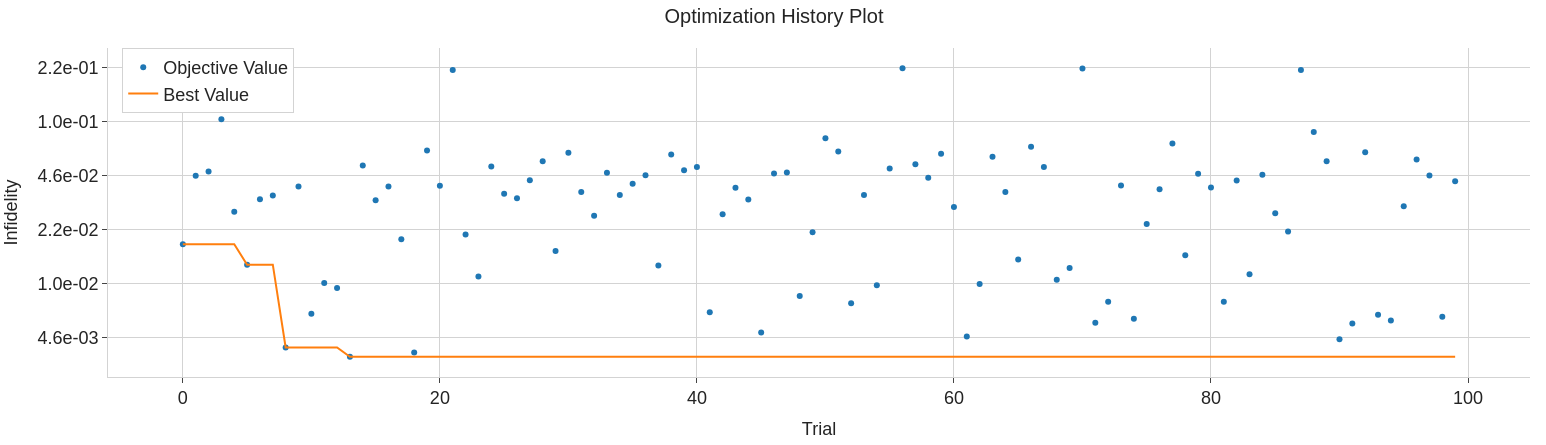
\includegraphics[width=\textwidth]{figures/png/RB_optimization/Optuna/100/optimization.png}
    \caption{Plot of the optimization history using \tt{Optuna} for 100 trials. Infidelity as a function of trials.}
    \label{fig:optuna100:optimization}
\end{figure}

\begin{figure}[h!]
    \centering
    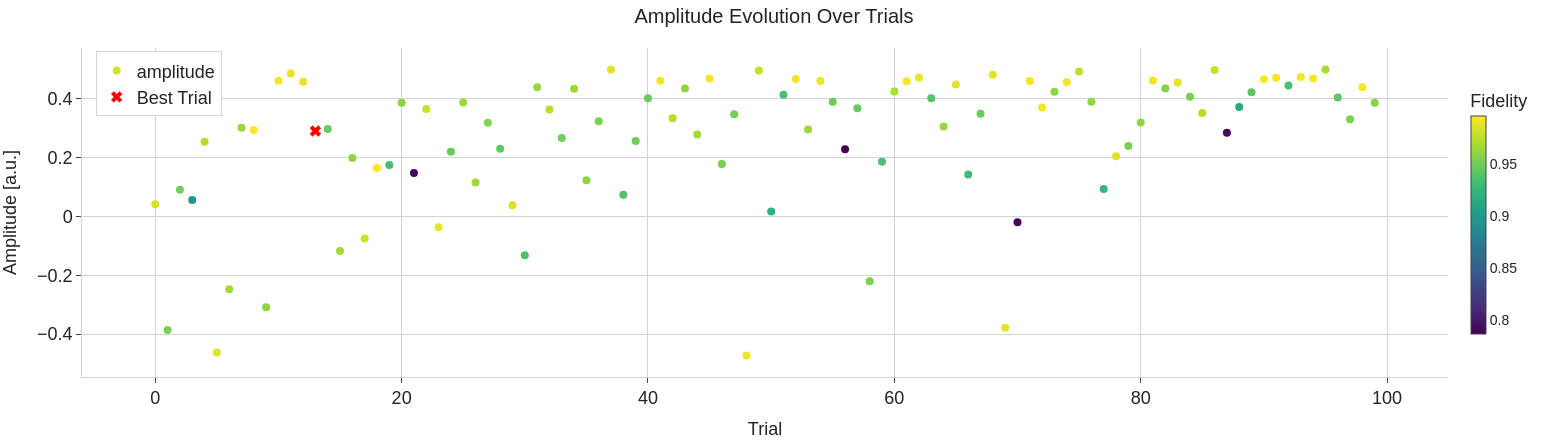
\includegraphics[width=\textwidth]{figures/png/RB_optimization/Optuna/100/amplitude.png}
    \caption{Plot of the $R_X(\pi)$ amplitude as a function of the number of trials.
    The color map indicates the Clifford gate average fidelity.
    The red cross denotes the $R_X(\pi)$ amplitude corresponding to the highest observed fidelity.}
    \label{fig:optuna100:amplitude}
\end{figure}

\begin{figure}[h!]
    \centering
    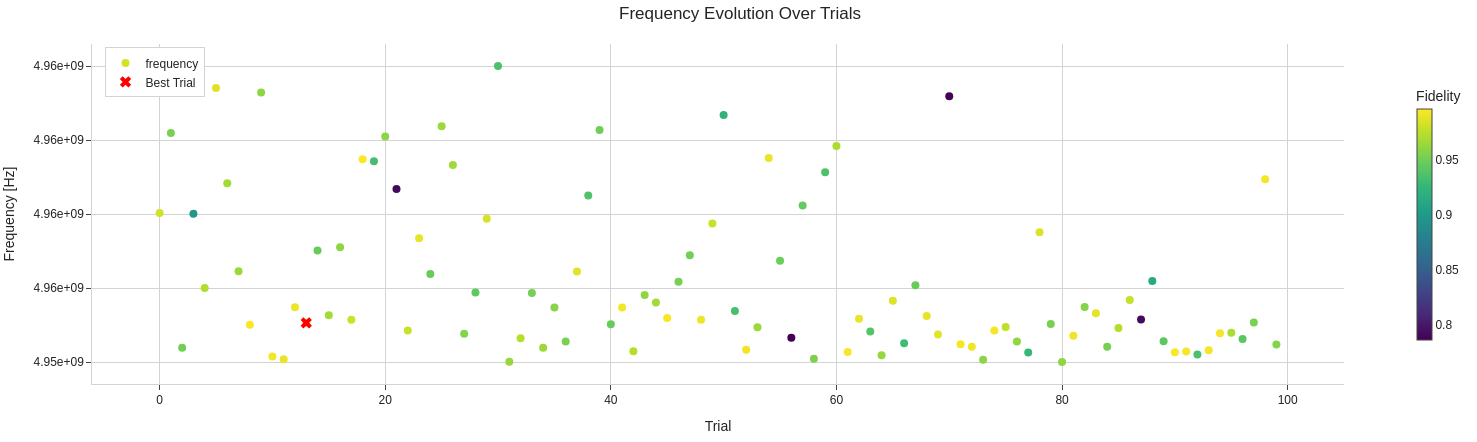
\includegraphics[width=\textwidth]{figures/png/RB_optimization/Optuna/100/frequency.png}
    \caption{Plot of the $R_X(\pi)$ frequency as a function of the number of trials. 
    The color map indicates the Clifford gate average fidelity.  
    The red cross denotes the $R_X(\pi)$ frequency corresponding to the highest observed fidelity.}
    \label{fig:optuna100:frequency}
\end{figure}

\begin{figure}[h!]
    \centering
    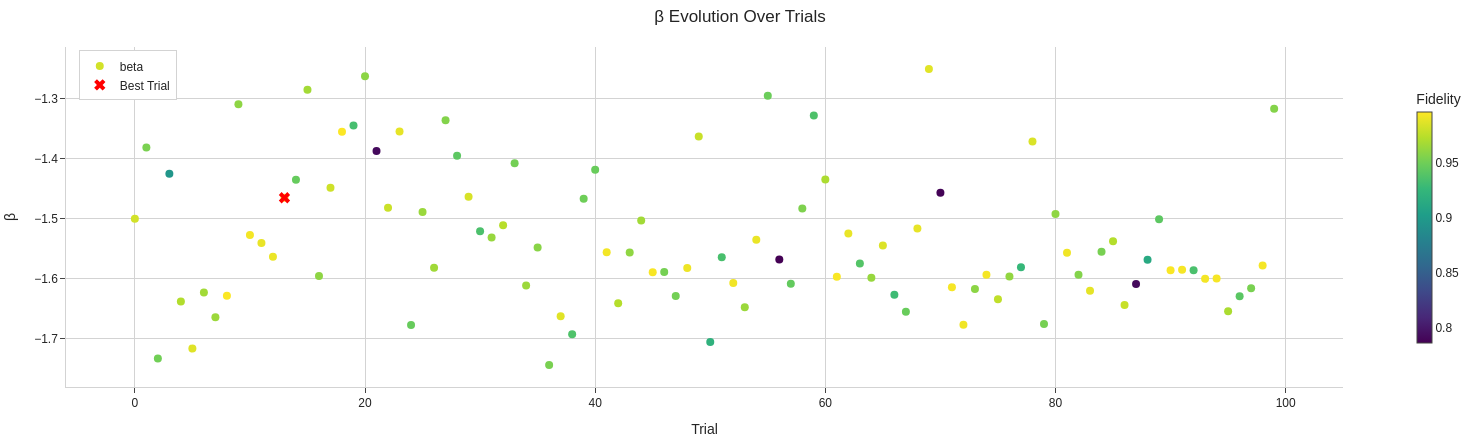
\includegraphics[width=\textwidth]{figures/png/RB_optimization/Optuna/100/beta.png}
    \caption{Plot of the value of the $\beta$ coefficient for the second quadrature of the $R_X(\pi)$ pulse as a function of the number of trials. 
    The color map indicates the Clifford gate average fidelity.  
    The red cross denotes the $\beta$ value corresponding to the highest observed fidelity}
    \label{fig:optuna100:beta}
\end{figure}

An analysis of the plots and the numerical values obtained for the $R_X(\pi)$ pulse parameters shows that the highest Clifford gate average fidelity corresponds to distinct values of these parameters. 
This effect is particularly evident for the amplitude and $\beta$ parameters. 
While the amplitude range remains fixed, being constrained by hardware limitations, the range used to search for the optimal $\beta$ varies significantly across the two optimization runs.

Although $\beta$ is not the most critical parameter in determining the fidelity outcome, as highlighted also by the Optuna analysis, which indicates that $\beta$ accounts on average for approximately 9\% of the fidelity improvement, 
its proper calibration does have a measurable impact on the shape of the control pulse and, therefore, on the overall gate performance.

The reason for the significant variation in the allowed search ranges for $\beta$ was then traced back to a failure in the fine-tuning routine responsible for calibrating the DRAG parameter.
The failed fitting routines are shown in Figure \ref{fig:failed_beta}. 
As a result of this issue, the optimization workflow was modified to include control on the $\chi^2$ value obtained from the fitting procedure to monitor potential failures in the pre-optimization stage.

\begin{figure}[h!]
    \centering
    \begin{subfigure}[t]{\textwidth}
        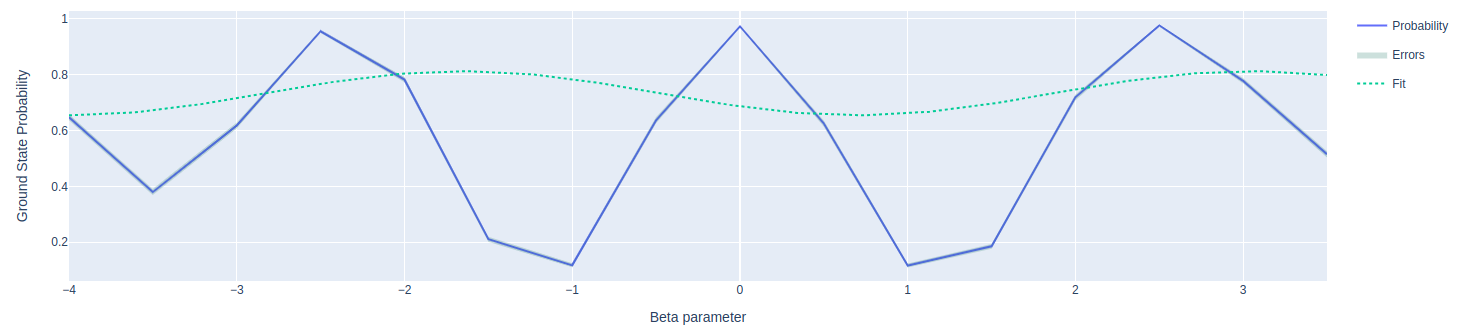
\includegraphics[width=\textwidth]{figures/png/RB_optimization/beta30.png}
        \caption{Plot of the output of the \tt{drag\_tuning} routine performed before running the 30 steps optimization with \tt{Optuna}.}
        \label{fig:failed_beta:30}
    \end{subfigure}
    \vspace{0.3cm}
    \begin{subfigure}[t]{\textwidth}
        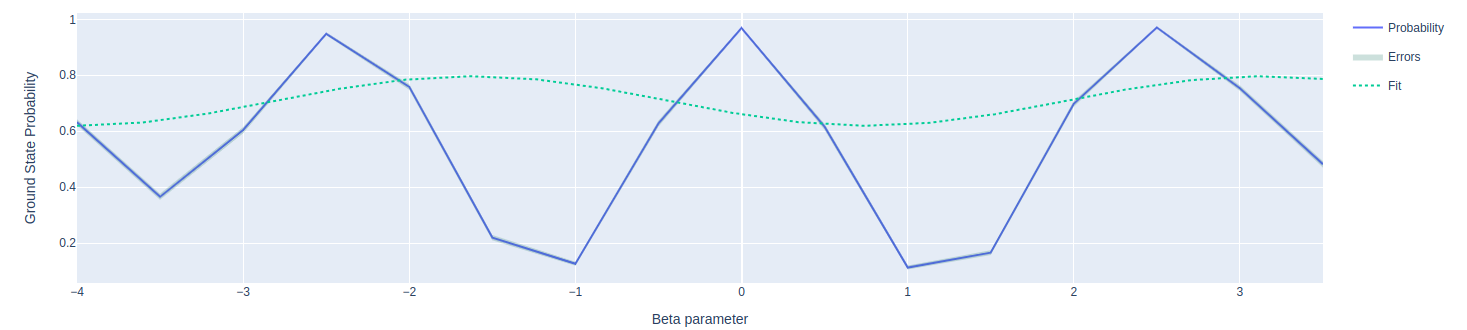
\includegraphics[width=\textwidth]{figures/png/RB_optimization/beta100.png}
        \caption{Plot of the output of the \tt{drag\_tuning} routine performed before running the 100 steps optimization with \tt{Optuna}.}
        \label{fig:failed_beta:100}
    \end{subfigure}

    \caption{Plots failed fine-tuning routines for estimating the $\beta$ parameter for the DRAG pulse shape. 
    From the plot is clear that the fitting procedure failed, a possible improvement to allow for a better fit could have been the choice of a smaller step size to scan the possible $\beta$ values.}
    \label{fig:failed_beta}
\end{figure}

%1000 steps
Given the results obtained in the two previous optimization runs using \tt{Optuna}, we proceeded with a third round of optimization, this time ensuring control over the execution of the fine-tuning routines that precede the optimization itself. 
In consideration of the relatively short time required by \tt{Optuna} in the previous attempt, approximately 40 minutes for 100 trials, we decided to significantly increase the number of optimization trials. 
Specifically, we set an upper limit of 1000 trials, to improve parameter space exploration and again potentially achieve better convergence.

The optimization history is shown in Figure \ref{fig:optuna1000beta:optimization}. 
At first, the results appear promising: the algorithm seems to achieve an average Clifford gate fidelity of 99.99\%. 
However a closer examination of the outputs corresponding to all RB routines with reported average Clifford gate infidelities below $1.5 \cdot 10^{-3}$, it becomes evident that these results are actually the consequence of failed exponential fits on the RB output.

Figure \ref{fig:RBfailed} presents a few representative examples of such cases, specifically showing the RB plots corresponding to the four lowest infidelities obtained during the optimization.

\begin{figure}[h!]
    \centering
    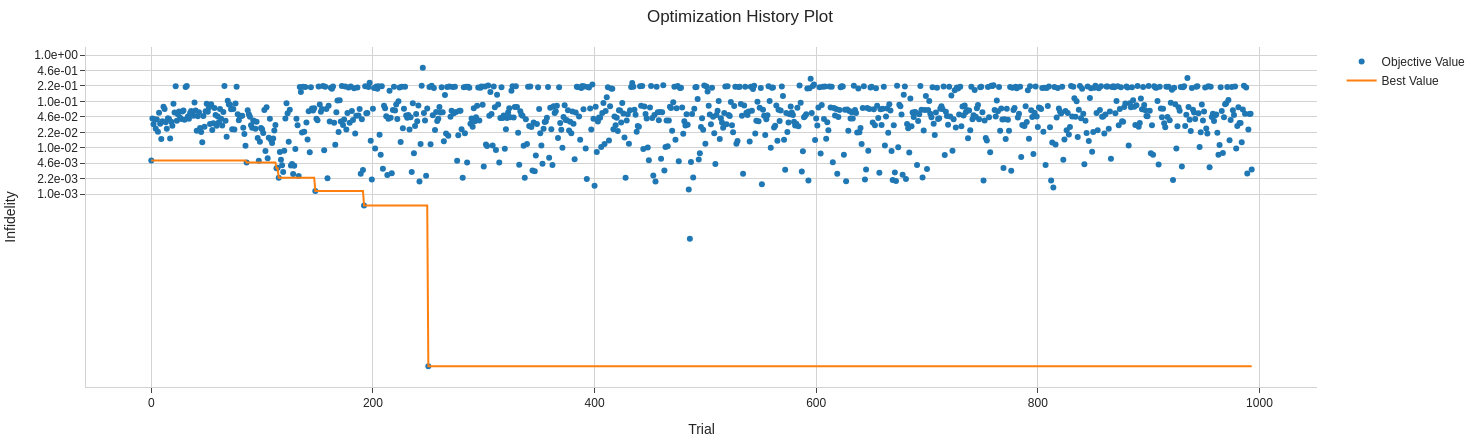
\includegraphics[width=\textwidth]{figures/png/RB_optimization/Optuna/1000beta/optimization.png}
    \caption{Plot of the optimization history using \tt{Optuna} for 1000 trials. Infidelity as a function of trials.}
    \label{fig:optuna1000beta:optimization}
\end{figure}

\begin{figure}[h!]
    \centering
    \begin{subfigure}[t]{0.495\textwidth}
        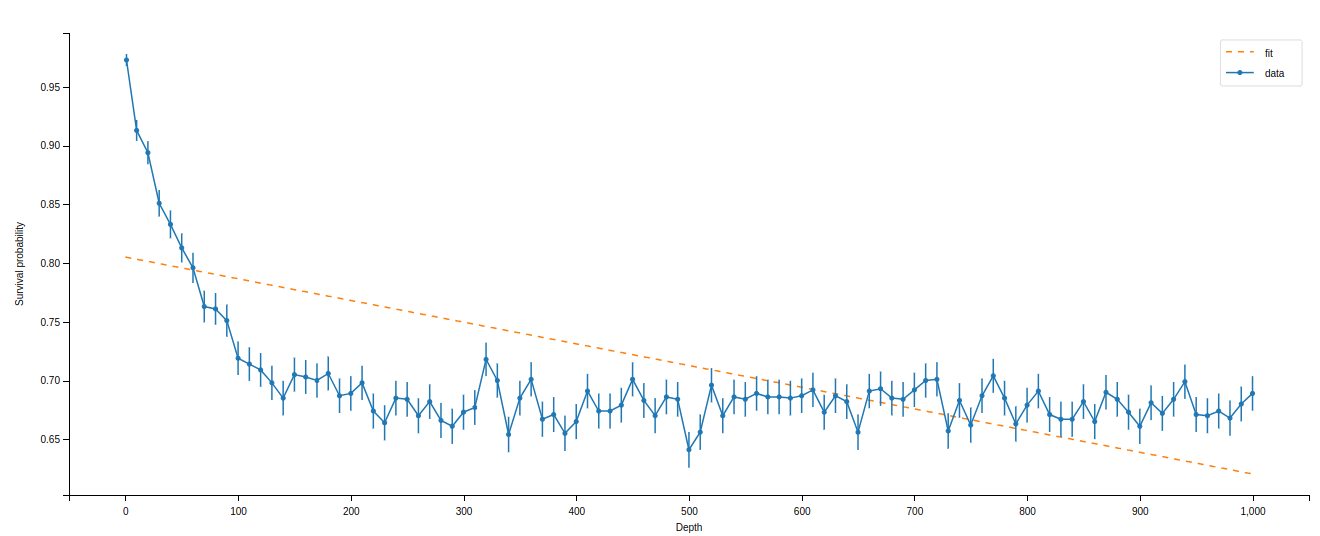
\includegraphics[width=\textwidth]{figures/png/RB_optimization/Optuna/1000beta/failed1.png}
        \caption{Plot of the output of RB protocol for trial 250.}
        \label{fig:optuna1000beta:failed1}
    \end{subfigure}
    \hfill
    \begin{subfigure}[t]{0.495\textwidth}
        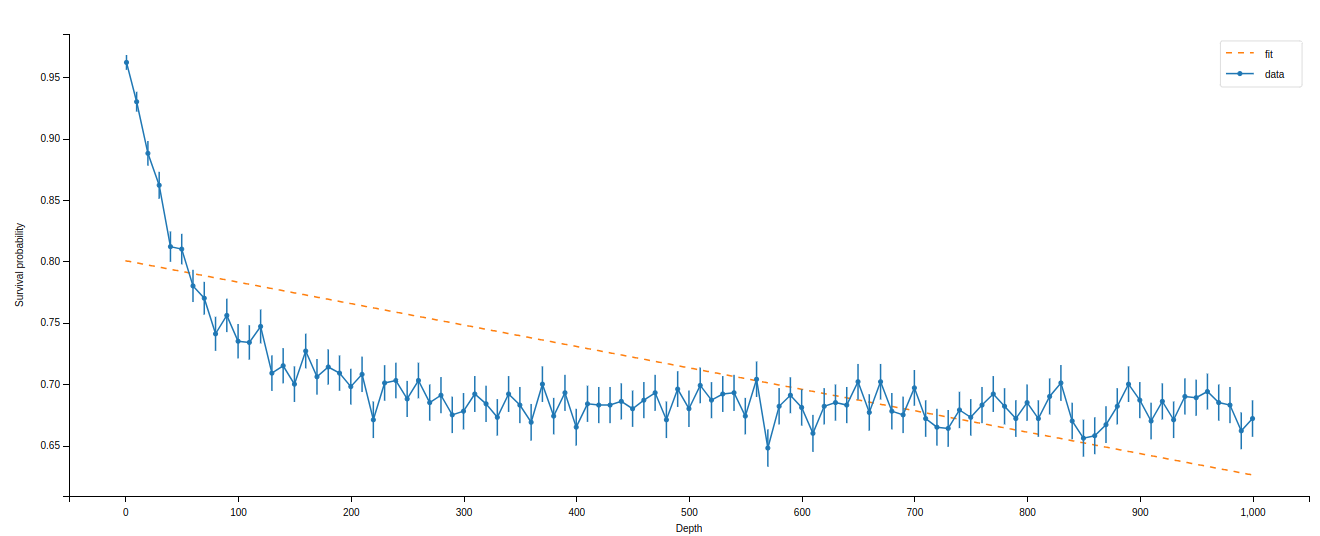
\includegraphics[width=\textwidth]{figures/png/RB_optimization/Optuna/1000beta/failed2.png}
        \caption{Plot of the output of RB protocol for trial 486.}
        \label{fig:optuna1000beta:failed2}
    \end{subfigure}

    \vspace{0.5cm}

    \begin{subfigure}[t]{0.495\textwidth}
        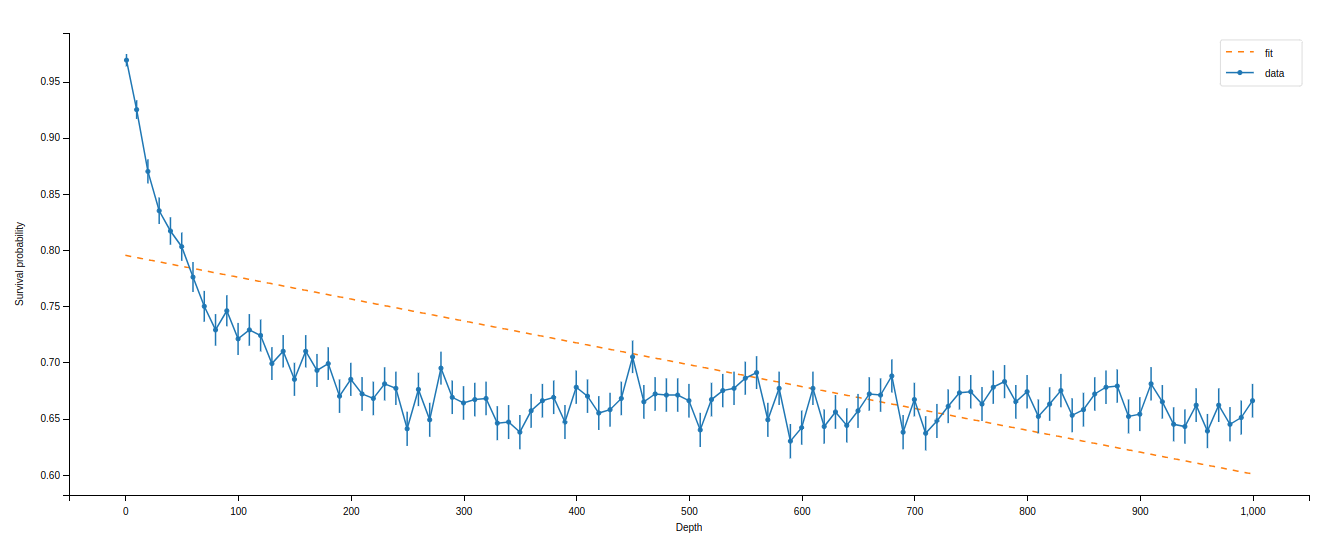
\includegraphics[width=\textwidth]{figures/png/RB_optimization/Optuna/1000beta/failed3.png}
        \caption{Plot of the output of RB protocol for trial 192.}
        \label{fig:optuna1000beta:failed3}
    \end{subfigure}
    \hfill
    \begin{subfigure}[t]{0.495\textwidth}
        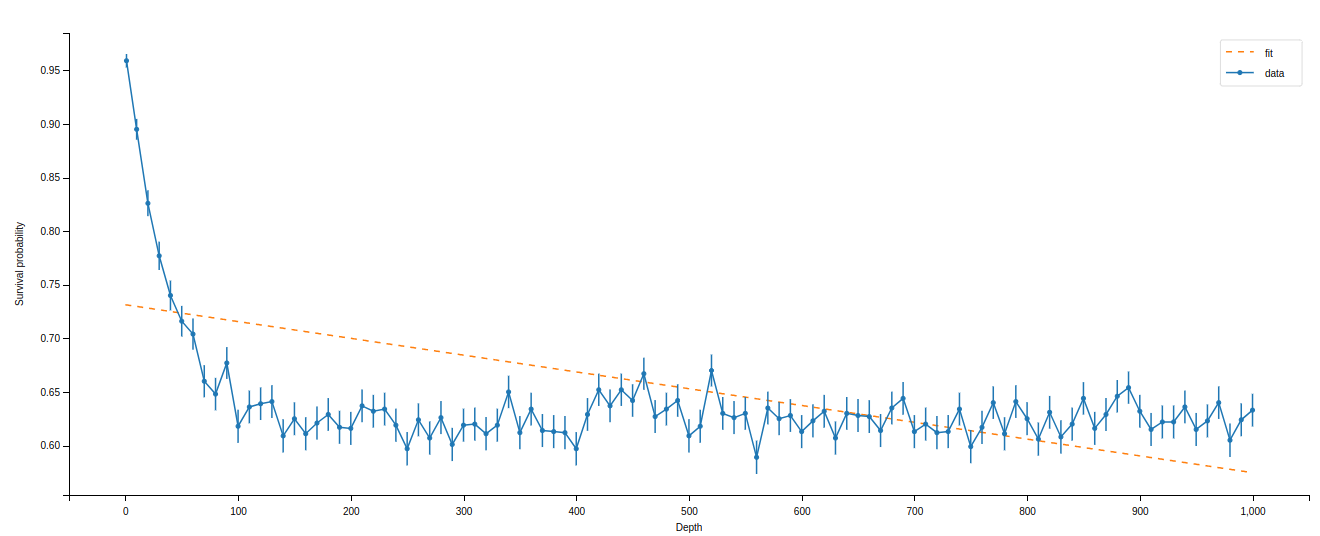
\includegraphics[width=\textwidth]{figures/png/RB_optimization/Optuna/1000beta/failed4.png}
        \caption{Plot of the output of RB protocol for trial 148.}
        \label{fig:optuna1000beta:failed4}
    \end{subfigure}

    \caption{Plots of the failed RB fit for different \tt{Optuna} trials.}
    \label{fig:RBfailed}
\end{figure}

At this point, the analysis was repeated after discarding all data points associated with a cost function value lower than $1.5 \cdot 10^{-3}$. 
The revised optimization history is shown in Figure \ref{fig:optuna1000beta:optimization_true}. 
In this analysis, the best fidelity achieved was 99.85\% much lower than the previously reported 99.98\%, but still a satisfactory result. 
This outcome corresponds to an improvement in fidelity of approximately 0.37\% compared to the initial configuration.

\begin{figure}[h!]
    \centering
    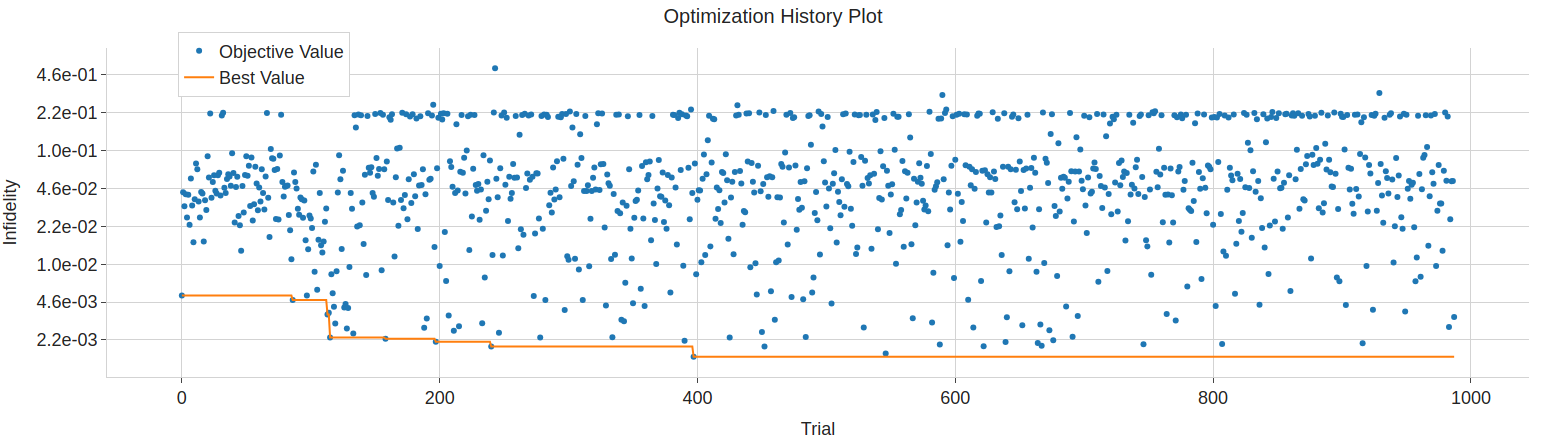
\includegraphics[width=\textwidth]{figures/png/RB_optimization/Optuna/1000beta/optimization_true.png}
    \caption{Plot of the optimization history using \tt{Optuna} for 1000 trials and excluding the data points associated to RB routines where the fitting procedure failed. 
    Infidelity as a function of trials.}
    \label{fig:optuna1000beta:optimization_true}
\end{figure}

\begin{figure}[h!]
    \centering
    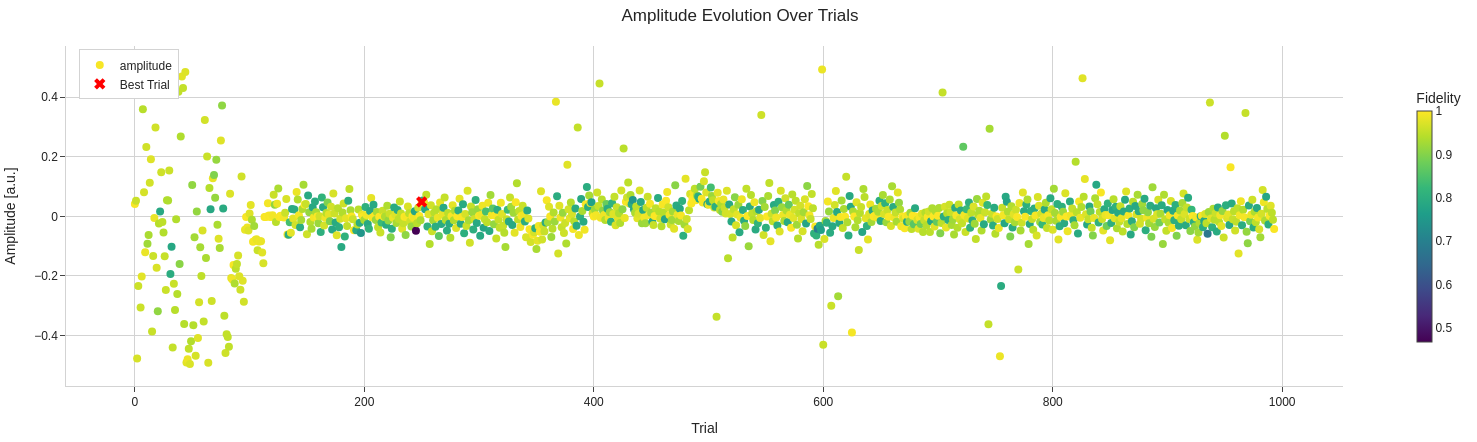
\includegraphics[width=\textwidth]{figures/png/RB_optimization/Optuna/1000beta/amplitude.png}
    \caption{Plot of the $R_X(\pi)$ amplitude as a function of the number of trials. 
    The colormap indicates the Clifford gate average fidelity. 
    The red cross denotes the $R_X(\pi)$ amplitude corresponding to the highest observed fidelity.}
    \label{fig:optuna1000beta:amplitude}
\end{figure}

\begin{figure}[h!]
    \centering
    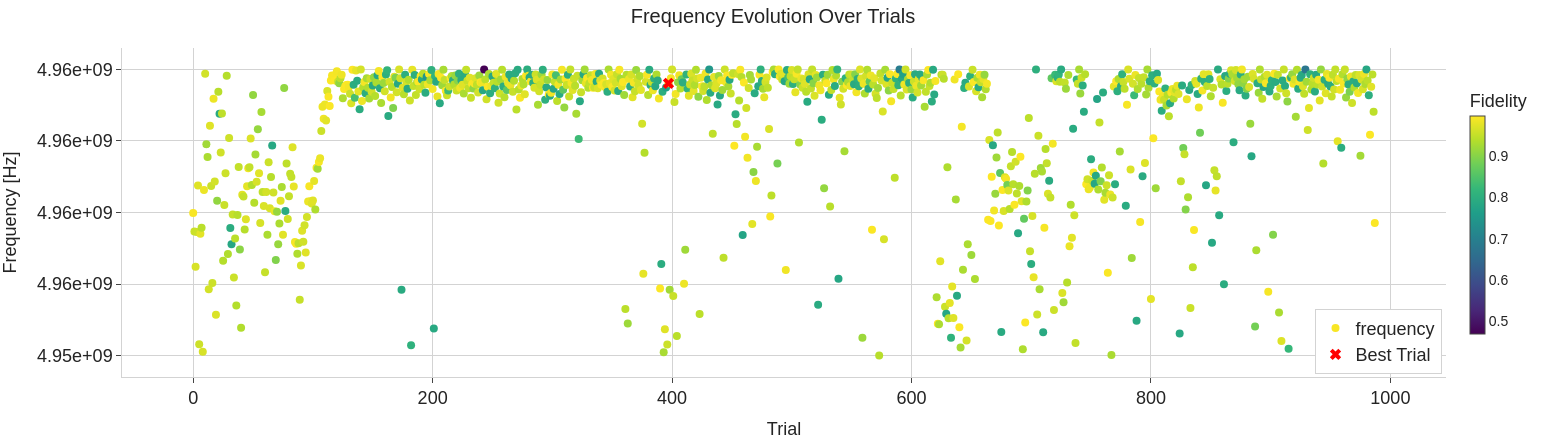
\includegraphics[width=\textwidth]{figures/png/RB_optimization/Optuna/1000beta/frequency.png}
    \caption{Plot of the $R_X(\pi)$ frequency as a function of the number of trials. 
    The colormap indicates the Clifford gate average fidelity.  
    The red cross denotes the $R_X(\pi)$ frequency corresponding to the highest observed fidelity.}
    \label{fig:optuna1000beta:frequency}
\end{figure}

\begin{figure}[h!]
    \centering
    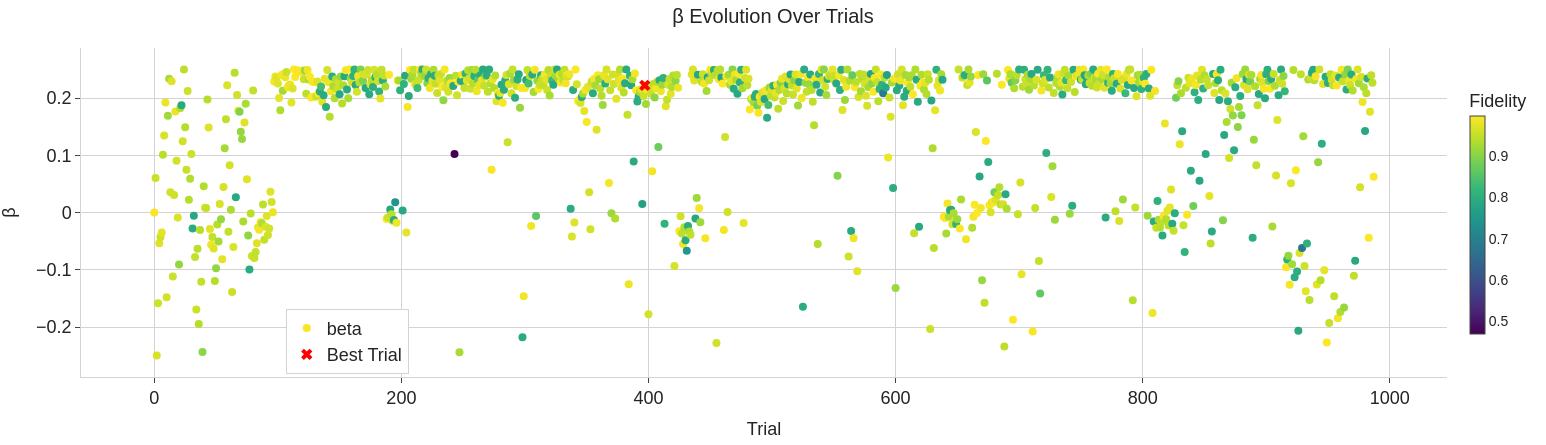
\includegraphics[width=\textwidth]{figures/png/RB_optimization/Optuna/1000beta/beta.png}
    \caption{Plot of the value of the $\beta$ coefficient for the second quadrature of the $R_X(\pi)$ pulse as a function of the number of trials. 
    The colormap indicates the Clifford gate average fidelity.  
    The red cross denotes the $\beta$ value corresponding to the highest observed fidelity}
    \label{fig:optuna1000beta:beta}
\end{figure}


%1000stepsnobeta
The evolution of the optimized parameters over the trials of the \tt{Optuna} run is shown in Figures \ref{fig:optuna1000beta:amplitude} - \ref{fig:optuna1000beta:beta}. 
Once again, the most interesting parameter to analyze is the DRAG coefficient $\beta$, whose sampled values are clearly centered around zero. 
Notably, the optimal value found for $\beta$ is approximately $-510 \cdot 10^{-6}$, a value so close to zero that it effectively corresponds to a purely Gaussian pulse shape.

As for the amplitude and frequency parameters, it is reassuring to observe that the best-performing values lie within the most densely sampled regions of the parameter space. 
This supports the conclusion that the optimization process executed by \texttt{Optuna} behaved as expected, effectively concentrating the search around the most promising areas.
Despite these observations, the system does not appear to be particularly stable, as small variations in the parameter values lead to significant fluctuations in the resulting fidelity. 
Overall, the results presented so far suggest that the optimization process carried out using \texttt{Optuna} does not exhibit clear convergence.

Based on the results obtained from the previous optimization run, particularly concerning the parameter $\beta$, a second optimization and measurement sequence was performed using the same configuration but varying only the amplitude and frequency of the $R_X(\pi)$ gate. 
The results of this new optimization run are presented in Figure \ref{fig:optuna1000:optimization}. 
In this case, the minimum of the cost function was reached at the 865\textsuperscript{th} step, corresponding to an average Clifford gate fidelity of 99.85\%.

This result is comparable to that obtained in the previous run, and it suggests two main conclusions. 
First, under the current fidelity regime, optimization over the parameter $\beta$ does not appear to play a significant role in improving performance. 
Second, it is likely that we have reached a saturation point in the cost landscape, where further improvements to the average Clifford gate fidelity cannot be achieved by tuning only the three parameters considered so far. 
This indicates that additional parameters or alternative control strategies may be required to surpass the current fidelity limit.

\begin{figure}[h!]
    \centering
    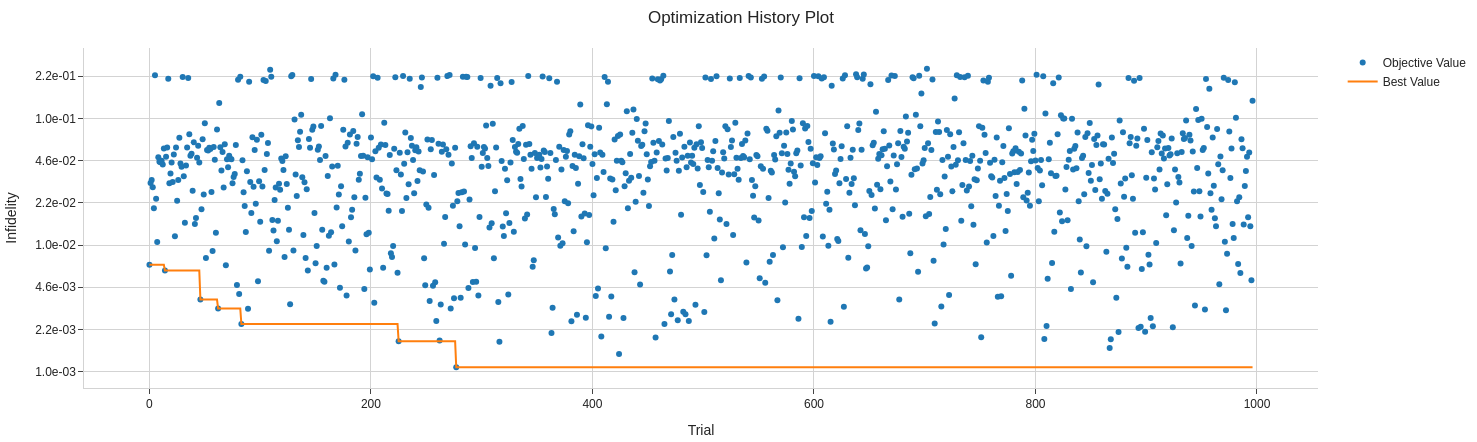
\includegraphics[width=\textwidth]{figures/png/RB_optimization/Optuna/1000/optimization.png}
    \caption{Plot of the optimization history using \tt{Optuna} for 1000 trials. Infidelity as a function of trials.}
    \label{fig:optuna1000:optimization}
\end{figure}

\begin{figure}[h!]
    \centering
    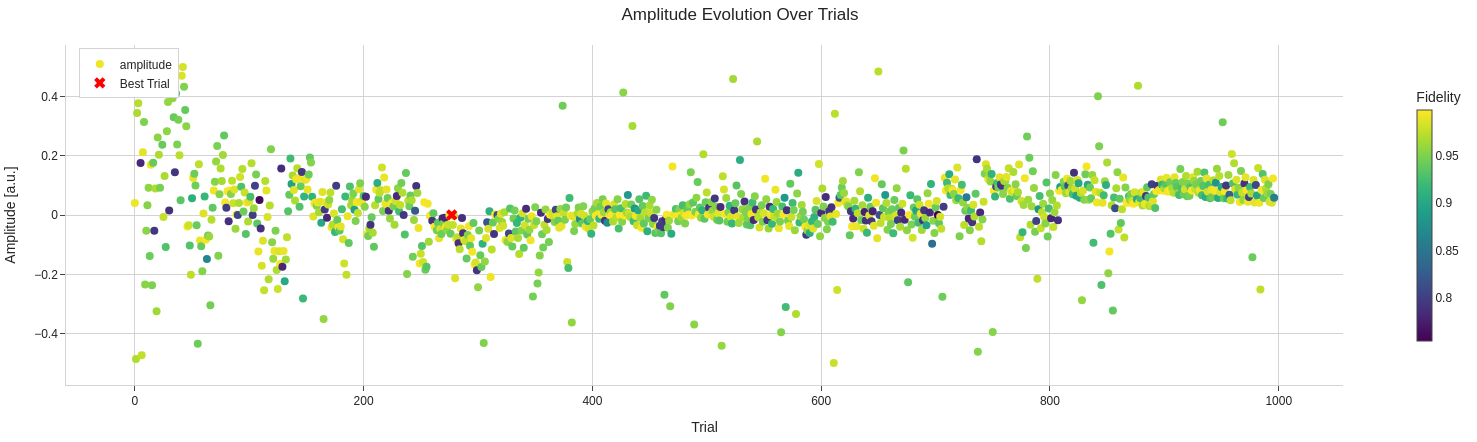
\includegraphics[width=\textwidth]{figures/png/RB_optimization/Optuna/1000/amplitude.png}
    \caption{Plot of the $R_X(\pi)$ amplitude as a function of the number of trials.     
    The colormap indicates the Clifford gate average fidelity. 
     The red cross denotes the $R_X(\pi)$ amplitude corresponding to the highest observed fidelity.}
    \label{fig:optuna1000:amplitude}
\end{figure}

\begin{figure}[h!]
    \centering
    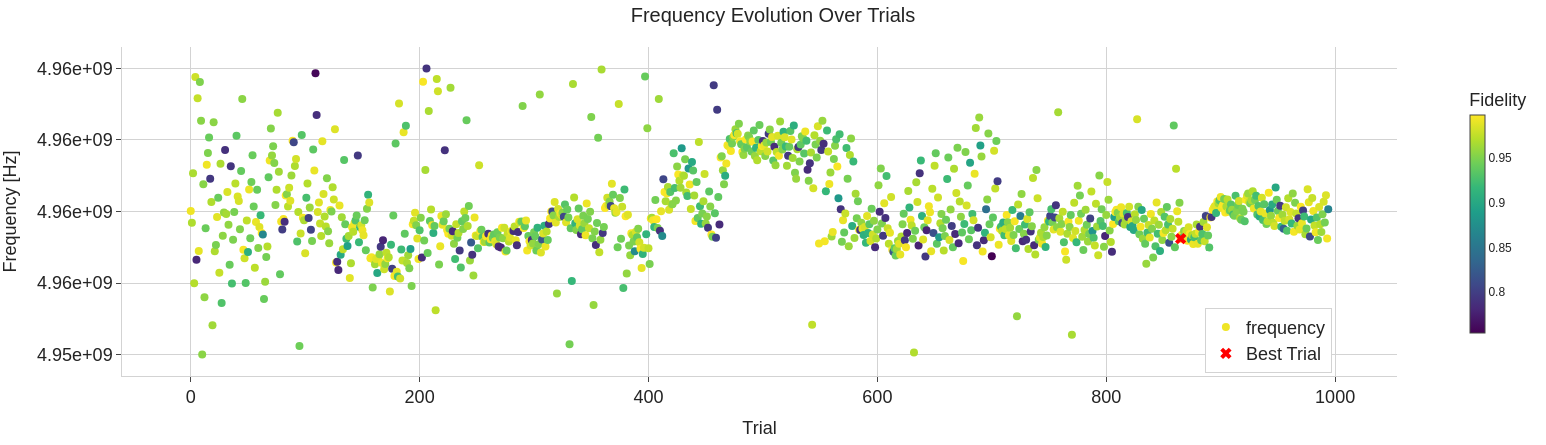
\includegraphics[width=\textwidth]{figures/png/RB_optimization/Optuna/1000/frequency.png}
    \caption{Plot of the $R_X(\pi)$ frequency as a function of the number of trials. 
    The colormap indicates the Clifford gate average fidelity.  
    The red cross denotes the $R_X(\pi)$ frequency corresponding to the highest observed fidelity.}
    \label{fig:optuna1000:frequency}
\end{figure}

The table below summarizes the infidelity values obtained at the final iteration for each of the optimization algorithms tested in this study. 
It also reports the number of optimization steps and function evaluations performed, as well as the total runtime required to complete each optimization.

\begin{table}[h]
    \centering
    \begin{tabular}{lcccccc}
        \toprule
        \textbf{Method} & \textbf{RB Value} & \textbf{Iterations} & \textbf{RB Evaluations} & \textbf{Duration [s]}\\
        \midrule
        \textbf{CMA-ES} & 0.003346 & 30 & 210 & 4 536 \\
        \textbf{Optuna 30 steps} & 0.018178  & 30 & 30 & 763\\
        \textbf{Optuna 100 steps} & 0.042908 & 100 & 100 & 2 257\\
        \textbf{Optuna 1000 steps} & 0.003424 & 1000 & 1000 & 21 811\\
        \textbf{Optuna no $\beta$} & 0.137907 & 1000 & 1000 & 21 820\\
        \bottomrule
    \end{tabular}
    \caption{This table provides a short summary of the results obtained using the \tt{CMA-ES} and \tt{Optuna} algorithm.\\ 
    In particular, regarding the \tt{Optuna} optimization algorithm the number of optimization iterations and of Randomized Benchmarking optimization is the same as the number of function evaluations coincides with the number of trials and no pruning was performed.
    The reported value of the objective function corresponds to the average Clifford gate infidelity obtained at the end of optimization via Randomized Benchmarking (1-fidelity), which serves as the cost function minimized by the algorithm.
    The \textit{Duration} column refers to the total runtime of the script, including the initial fine-tuning stage preceding the optimization.\\}
    \label{tab:optuna_opt}
\end{table}

\section{RB optimization conclusions}

As outlined at the beginning of this chapter, the primary goal was to evaluate whether an automated optimization procedure—executed directly on quantum hardware—could reliably improve the average fidelity of single-qubit Clifford gates, specifically the $R_X(\pi)$ gate. 
The desired outcome was a routine that could be executed periodically, improving gate fidelity in a reproducible and time-efficient manner.

The results obtained from various optimization strategies, Nelder-Mead, \tt{CMA-ES}, and \tt{Optuna}, demonstrate that while meaningful improvements in fidelity are achievable, the current implementation does not yet meet the robustness and efficiency requirements for routine deployment. 
The primary bottleneck remains the cost of the Randomized Benchmarking (RB) routine, which is necessary for fidelity evaluation. 
Because each optimization requires multiple evaluations of this cost function, the total execution time quickly becomes a limiting factor.

Additionally, we found that convergence is not guaranteed. 
In several cases, especially those involving \tt{Optuna} or \tt{CMA-ES} with a broader parameter search, the optimization did not yield stable or reproducible results.
Even when high fidelities were reached (up to 99.85\%), the fidelity showed large sensitivity to small changes in parameter values, casting doubt on the practical stability of the identified configurations.
This is particularly evident from the results shown in Table \ref{tab:best_param} and illustrated in Figure \ref{fig:params_best}.

\begin{figure}[h!]
    \centering
    \begin{subfigure}[t]{0.3\textwidth}
        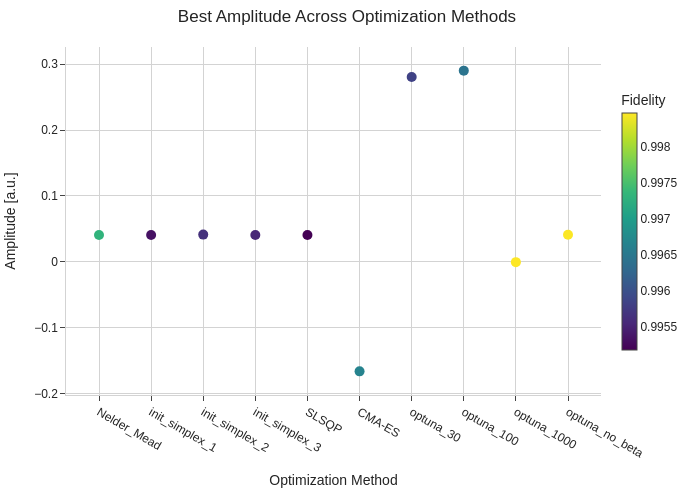
\includegraphics[width=\textwidth]{figures/png/RB_optimization/BestAmplitude.png}
        \caption{Amplitude values corresponding to highest fidelity for each optimization method.}
        \label{fig:amplitude_best}
    \end{subfigure}
    \hfill
    \begin{subfigure}[t]{0.3\textwidth}
        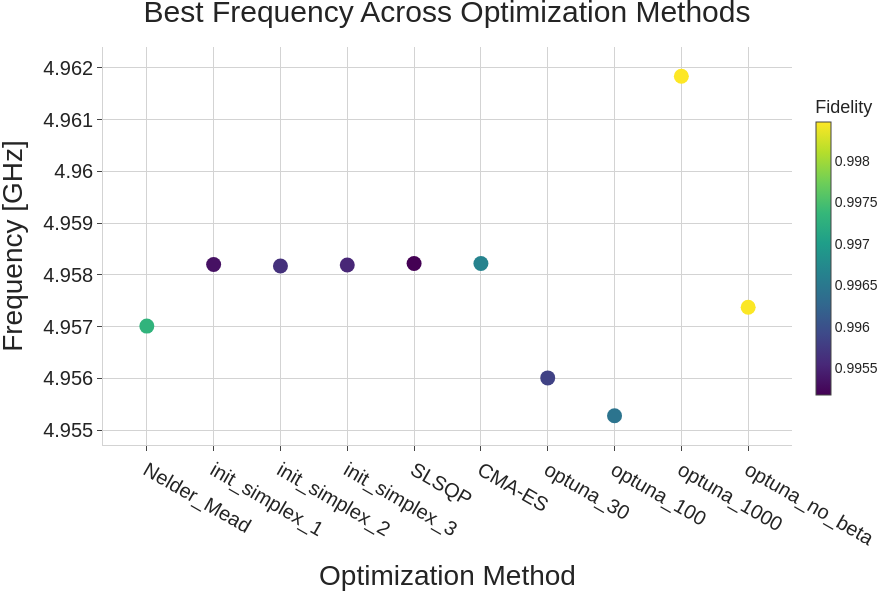
\includegraphics[width=\textwidth]{figures/png/RB_optimization/BestFrequency.png}
        \caption{Frequency values corresponding to highest fidelity for each optimization method.}
        \label{fig:frequency_best}
    \end{subfigure}
    \hfill
    \begin{subfigure}[t]{0.3\textwidth}
        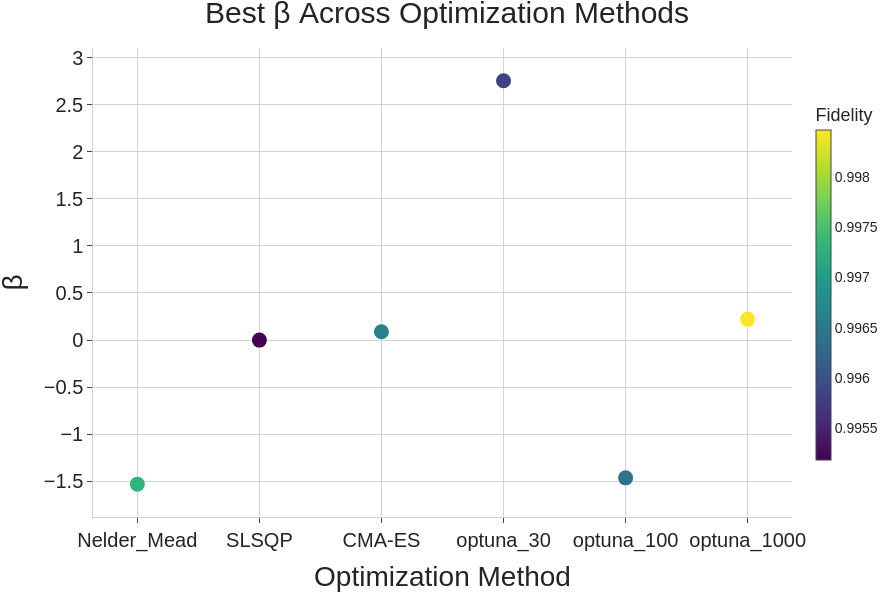
\includegraphics[width=\textwidth]{figures/png/RB_optimization/BestBeta.png}
        \caption{Values of the $\beta$ parameter corresponding to highest fidelity for each optimization method.
        The cases in which the $\beta$ parameter was not updated during the optimization are not reported.}
        \label{fig:beta_best}
    \end{subfigure}
    \caption{The plots show the best parameter values for the different optimization methods tested.} 
    \label{fig:params_best}
\end{figure}

\begin{table}[h]
    \centering
    \begin{tabular}{lcccc}
        \toprule
        \textbf{Analysis} & \textbf{Fidelity} & \textbf{Amplitude [a.u.]} & \textbf{Frequency} & \textbf{$\beta$} \\
        \textbf{Name} & \textbf{Best} & \textbf{Amplitude [a.u.]} & \textbf{Best [$\times10^9$ Hz]} & \textbf{Best} \\
        \midrule
        \textbf{Nelder\_Mead} & 0.99731 & 0.04063 & 4.95701 & -1.53253 \\
        \textbf{init\_simplex\_1} & 0.99533 & 0.04069 & 4.95820 & - \\
        \textbf{init\_simplex\_2} & 0.99564 & 0.04131 & 4.95817 & - \\
        \textbf{init\_simplex\_3} & 0.99554 & 0.04058 & 4.95819 & - \\
        \textbf{SLSQP} & 0.99518 & 0.04058 & 4.95822 & -0.00115 \\
        \textbf{CMA-ES} & 0.99665 & -0.16634 & 4.95822 & 0.08802 \\
        \textbf{optuna\_30} & 0.99583 & 0.28059 & 4.95601 & 2.75519 \\
        \textbf{optuna\_100} & 0.99645 & 0.29026 & 4.955279 & -1.46504 \\
        \textbf{optuna\_1000} & 0.99847 & -0.00051 & 4.961836 & 0.2222 \\
        \textbf{optuna no $\beta$} & 0.99846 & 0.04104 & 4.957374 & - \\
        \bottomrule
    \end{tabular}
    \caption{The table reports the best fidelity, amplitude, frequency, and $\beta$ from each optimization method allowing for an easy comparison.}
    \label{tab:best_param}
\end{table}

Two directions for future improvement emerge from this work. 
First, the RB evaluation process itself could be optimized. 
In the present study, sequences of depth 1000 were used, and for each depth, 1000 Clifford circuits were sampled. 
This approach, while reliable, is computationally expensive. 
A detailed study, possibly involving hyperparameter optimization techniques, could help determine whether shorter sequences or fewer samples still yield meaningful fidelity estimates, potentially reducing total runtime and making on-chip calibration more feasible.

Second, the performance of the optimization algorithms themselves could be refined. 
For example, in the case of \tt{CMA-ES}, adjusting the population size or reducing the initial value of $\sigma$ could improve convergence, albeit at the cost of reduced parameter space exploration or increased computational load. 
These modifications may be particularly relevant in a more stable calibration regime, where parameter values show limited drift over time.

Another promising direction, particularly with \tt{Optuna}, would be to adopt a multi-objective optimization strategy, where both fidelity and optimization time are minimized simultaneously. 
However, this approach was not pursued in this work due to the instability of the fidelity results observed even in high-trial regimes, highlighting the current limitations of fidelity optimization using this method.

In conclusion, while the results suggest that automated, hardware-level gate fidelity optimization is feasible in principle, substantial improvements are still needed in both the fidelity evaluation routine and the optimization algorithm design before such a protocol can be adopted for regular use on our quantum hardware.

\begin{sidewaystable}[h]
    \centering
    \begin{tabular}{lccccccccccc}
        \toprule
        \textbf{Analysis} & \textbf{Initial} & \textbf{Best} & \textbf{Best} & \textbf{Amplitude} & \textbf{Frequency} & \textbf{$\beta$} & \textbf{Best cost} & \textbf{Initial} & \textbf{Best} & \textbf{Best fidelity} \\
        \textbf{Name} & \textbf{cost} & \textbf{cost} & \textbf{index} & \textbf{best [a.u.]} & \textbf{ best [$\times10^9$ Hz]} & \textbf{best} & \textbf{improv. [\%]} & \textbf{fidelity} & \textbf{fidelity} & \textbf{improv[\%]} \\
        \midrule
        \textbf{Nelder\_Mead} & 0.00983 & 0.00269 & 19 & 0.04063 & 4.95701 & -1.53253 & 72.59 & 0.99017 & 0.99731 & 0.72 \\
        \textbf{init\_simplex\_1} & 0.00633 & 0.00467 & 25 & 0.04069 & 4.95820 & - & 26.23 & 0.99367 & 0.99533 & 0.17 \\
        \textbf{init\_simplex\_2} & 0.00607 & 0.00436 & 17 & 0.04131 & 4.95817 & - & 28.27 & 0.99393 & 0.99564 & 0.17 \\
        \textbf{init\_simplex\_3} & 0.00585 & 0.00446 & 37 & 0.04058 & 4.95819 & - & 23.73 & 0.99415 & 0.99554 & 0.14 \\
        \textbf{SLSQP} & 0.02172 & 0.00482 & 13 & 0.04058 & 4.95822 & -0.00115 & 77.79 & 0.97828 & 0.99518 & 1.73 \\
        \textbf{CMA-ES} & 0.00728 & 0.00335 & 9 & -0.16634 & 4.95822 & 0.08802 & 54.04 & 0.99272 & 0.99665 & 0.40 \\
        \textbf{optuna\_30} & 0.016471 & 0.00416 & 23 & 0.28059 & 4.95601 & 2.75519 & 74.70 & 0.98352 & 0.99583 & 1.25 \\
        \textbf{optuna\_100} & 0.017535 & 0.00354& 13 & 0.29026 & 4.955279 & -1.46504 & 79.77 & 0.98246 & 0.99645 & 1.42\\
        \textbf{optuna\_1000} & 0.005307 & 0.00152 & 405 & -0.00051 & 4.961836 & 0.2222 & 71.18 & 0.99469 & 0.99847 & 0.37\\
        \textbf{optuna no $\beta$} & 0.006983 & 0.00153 & 865 & 0.04104 & 4.957374 & - & 77.96 & 0.99301 & 0.99846 & 0.54\\
        \bottomrule
    \end{tabular}
    \caption{This table reports the results obtained from the optimization of the average Clifford gate fidelity as a function of the pulse frequency, amplitude, and the parameter $\beta$, which scales the second quadrature component in the case of a DRAG pulse.
    Specifically, it shows the initial and optimal values of the cost function, as well as the corresponding parameter values at the optimum. 
    The table also includes the initial fidelity, the percentage decrease in the cost function, and the percentage improvement in fidelity achieved after optimization.}
    \label{tab:best_values}
\end{sidewaystable}

\begin{sidewaystable}[h]
    \centering
    \begin{tabular}{lcccccccccc}
        \toprule
        \textbf{Analysis} & \textbf{Initial} & \textbf{Final} & \textbf{Amplitude} & \textbf{Frequency} & \textbf{$\beta$} & \textbf{Final cost} & \textbf{Initial} & \textbf{Final} & \textbf{Final fidelity} \\
        \textbf{Name} & \textbf{cost} & \textbf{cost} & \textbf{final [a.u.]} & \textbf{final [$\times10^9$ Hz]} & \textbf{final} & \textbf{improv. [\%]} & \textbf{fidelity} & \textbf{fidelity} & \textbf{improv. [\%]} \\
        \midrule
        \textbf{Nelder\_Mead} & 0.00983 & 0.00295 & 0.04067 & 4.95699 & -1.53976 & 70.02 & 0.99017 & 0.99705 & 0.69 \\
        \textbf{init\_simplex\_1} & 0.00633 & 0.00517 & 0.04069 & 4.95820 & - & 18.41 & 0.99367 & 0.99483 & 0.12 \\
        \textbf{init\_simplex\_2} & 0.00607 & 0.00437 & 0.04132 & 4.95817 & - & 28.10 & 0.99393 & 0.99563 & 0.17 \\
        \textbf{init\_simplex\_3} & 0.00585 & 0.00512 & 0.04058 & 4.95819 & - & 12.46 & 0.99415 & 0.99488 & 0.07 \\
        \textbf{SLSQP} & 0.02172 & 0.00507 & 0.04058 & 4.95822 & -0.00115 & 76.64 & 0.97828 & 0.99493 & 1.70 \\
        \textbf{CMA-ES} & 0.00728 & 0.003346 & 0.12956 & 4.95822 & 0.18364 & -265.93 & 0.99272 & 0.97336 & -1.95 \\
        \textbf{optuna\_30} & 0.016471 & 0.018178 & 0.46076 & 4.95479 & 2.92767 & -10.36 & 0.98352 & 0.98182 & -0.17\\
        \textbf{optuna\_100} & 0.017535 & 0.042908 &  0.386175 & 4.95469 & -1.31692 & -144.68 & 0.98246 & 0.95709 & -2.58\\
        \textbf{optuna\_1000} & 0.005307 & 0.003424 & -0.042718 & 4.95794 & 0.0626649 & 35.48 & 0.99469 & 0.99657 & 0.18\\
        \textbf{optuna no $\beta$} & 0.006983 & 0.137907 & 0.058214 & 4.95818 & - & -1874.74 & 0.99301 & 0.86209 & -13.18\\
        \bottomrule
    \end{tabular}
    \caption{This table reports the results obtained from the optimization of the average Clifford gate fidelity as a function of the pulse frequency, amplitude, and the parameter $\beta$, which scales the second quadrature component in the case of a DRAG pulse.
    Specifically, it shows the initial and final values of the cost function, as well as the corresponding parameter values at the final step. 
    The table also includes the initial fidelity, the percentage decrease in the cost function, and the percentage improvement in fidelity achieved at the end of the optimization process.}
    \label{tab:final_values}
\end{sidewaystable}

%TODO: inserire riferimento all'appendice in cui mostro tutte le valutazioni che faccio della fidelity